\documentclass[11pt,a4paper]{article}
\usepackage[T1]{fontenc}
\usepackage[utf8]{inputenc}
\usepackage{lmodern,microtype}
\usepackage{amsmath,amssymb,amsthm,mathtools}
\usepackage{booktabs,array,enumitem}
\usepackage[margin=27mm]{geometry}
\usepackage{tikz}
\usetikzlibrary{arrows.meta,positioning,calc,shapes.geometric,decorations.pathreplacing}
\usepackage{listings}
\usepackage[colorlinks=true,linkcolor=blue!60!black,urlcolor=blue!60!black,citecolor=green!40!black]{hyperref}
\allowdisplaybreaks

\newtheorem{theorem}{Theorem}[section]
\newtheorem{lemma}[theorem]{Lemma}
\newtheorem{proposition}[theorem]{Proposition}
\newtheorem{corollary}[theorem]{Corollary}
\newtheorem{conjecture}[theorem]{Conjecture}
\newtheorem{imported}[theorem]{Imported theorem}
\theoremstyle{definition}
\newtheorem{definition}[theorem]{Definition}
\theoremstyle{remark}
\newtheorem{remark}[theorem]{Remark}
\newtheorem{example}[theorem]{Example}

\newtheorem*{mainA}{Theorem A (sharper universal constants)}
\newtheorem*{mainB}{Theorem B (whole-sketch Nystr\"om bound)}
\newtheorem*{mainC}{Theorem C (block drift and diagonal training)}
\newtheorem*{mainD}{Theorem D (adaptive frame selection)}
\newtheorem*{mainE}{Theorem E (sketched RPCholesky, imported)}

\newcommand{\E}{\mathbb E}
\newcommand{\Prob}{\mathbb P}
\newcommand{\R}{\mathbb R}
\newcommand{\C}{\mathbb C}
\newcommand{\tr}{\operatorname{tr}}
\newcommand{\diag}{\operatorname{diag}}
\newcommand{\rank}{\operatorname{rank}}
\newcommand{\range}{\operatorname{range}}
\newcommand{\eps}{\varepsilon}
\newcommand{\norm}[1]{\lVert#1\rVert}
\newcommand{\Nys}{\mathcal N}
\newcommand{\1}{\mathbf 1}
\newcommand{\T}{\mathsf T}
\newcommand{\proofstep}[1]{\par\medskip\noindent\textbf{#1}\enspace}
\newcommand{\Lbar}{\overline\Lambda}

\lstset{basicstyle=\ttfamily\footnotesize,columns=fullflexible,keepspaces=true,
  frame=single,breaklines=true,xleftmargin=1em,framexleftmargin=0.5em}

\title{SparseStack: sharper constants, whole-sketch Nystr\"om bounds,\\
and adaptive frame selection}
\author{}
\date{29 September 2026}

% Shared manuscript typography. Keep this file beside the manuscript folders.
\usepackage{needspace}
\usepackage{etoolbox}
\linespread{1.08}
\setlength{\parskip}{0.38em plus 0.08em minus 0.05em}
\setlength{\parindent}{1.25em}
\setlength{\emergencystretch}{2em}
\setlist{itemsep=4pt,topsep=6pt,parsep=2pt}
\renewcommand{\arraystretch}{1.16}
\setlength{\tabcolsep}{6pt}
\AtBeginDocument{%
  \setlength{\abovedisplayskip}{10pt plus 2pt minus 2pt}%
  \setlength{\belowdisplayskip}{10pt plus 2pt minus 2pt}%
  \setlength{\abovedisplayshortskip}{5pt plus 2pt}%
  \setlength{\belowdisplayshortskip}{8pt plus 2pt minus 2pt}%
}
\makeatletter
\def\th@plain{%
  \thm@preskip=10pt plus 2pt minus 2pt
  \thm@postskip=10pt plus 2pt minus 2pt
  \itshape
}
\def\th@definition{%
  \thm@preskip=10pt plus 2pt minus 2pt
  \thm@postskip=10pt plus 2pt minus 2pt
  \normalfont
}
\def\th@remark{%
  \thm@headfont{\itshape}%
  \thm@preskip=9pt plus 2pt minus 2pt
  \thm@postskip=9pt plus 2pt minus 2pt
  \normalfont
}
\makeatother
\AtBeginEnvironment{proof}{\Needspace{4\baselineskip}}
\widowpenalty=10000
\clubpenalty=10000
\displaywidowpenalty=10000
\raggedbottom


\begin{document}
\maketitle

\begin{abstract}
SparseStack can use fewer rows and fewer nonzeros per column without
changing its distribution or its operator proof. We sharpen an existing
all-order moment certificate from the universal constant pair
$(26.5,179)$ to $(25,154)$, with two alternative sparsity--row tradeoffs.
The improvement retains the relation between the dimension ratio and
the bucket count; all $63$ interval checks are certified in exact
rational arithmetic. We also prove a deterministic Nystr\"om bound
$\|R\|_F^2\le\operatorname{tr}(AZAZ)$ and compute its exact SparseStack
expectation, yielding $\mathbb E\|R\|_F^2\le2(\operatorname{tr}A)^2/m$.
A finite-support obstruction explains why this expected bound cannot be
uniformly relative to a spectral tail. Finally, we specialize convex
residual drift and diagonal estimation to independent CountSketch blocks,
and use classical adaptive-versus-volume sampling to justify sketch
reuse with a spectral selection price at most $k!$.
\end{abstract}

\tableofcontents

\section{Introduction}\label{sec:intro}

SparseStack is the sparse sketching matrix
\[
 \Pi=s^{-1/2}\begin{bmatrix}H_1\\ \vdots\\ H_s\end{bmatrix}\in\R^{m\times n},
 \qquad m=sb,
\]
built from $s$ independent CountSketch blocks $H_g\in\R^{b\times n}$
\cite{CharikarChenFarachColton2002,KaneNelson2014,NelsonNguyen2013}.
Every column has exactly $s$ nonzero entries $\pm s^{-1/2}$. The direct-model theorem of
\emph{Graded Multiplication Operators for Random-Matrix
Moments}~\cite[Theorem~10.6 and Appendix~B]{SS} proves the optimal oblivious subspace embedding (OSE) guarantee
$m=O((d+\log(1/\delta))/\eps^2)$, $s=O(\log(d/\delta)/\eps)$ with explicit
universal constants: $s<26.5\,q/\eps$ and $m<179(d+q)/\eps^2$, where
$q=\max\{1,\lceil\log_4(d/\delta)\rceil\}$. Its proof bounds the moment
$\E\tr E^{2q}$ of the Gram error $E=U^\T\Pi^\T\Pi U-I_d$ by the vacuum
entry of the $2q$-th power of a scalar tridiagonal majorant $T_q$, and
then bounds that entry by a single concave row-sum envelope.

This companion does three things with that machinery. First, it
sharpens the final scalar step: the envelope used in~\cite{SS} replaces a
dimension ratio by one while using only a fixed small lower bound on the
bucket count $b$. These two losses cannot both be worst-case, and
retaining their correlation improves both universal constants
(Section~\ref{sec:constants}). Second, it studies what SparseStack gives
for Nystr\"om approximation of a PSD matrix, where the natural quantity
is not an embedding of a fixed subspace but the whole Gram error
$Z=\Pi^\T\Pi-I_n$ (Sections~\ref{sec:nystrom} and~\ref{sec:blocks}).
Third, it treats sketch-dependent targets: a frame selected after seeing
the sketch by randomly pivoted Cholesky (RP), and RP run directly on the
sketched Gram matrix (Sections~\ref{sec:gate} and~\ref{sec:sketchedrp}).

\subsection{What improves, and what is inherited}\label{sec:main-results}
The central contribution is a sharper \emph{sufficient} parameter
prescription for the same real, fully independent sketch. Its operator
estimates are inherited and stated explicitly in Section~\ref{sec:model};
the new proof starts at the scalar envelope. The separate Nystr\"om,
drift, and selection results describe what can be deduced from the
sketch's moment structure. They make no claim of a new sketching
distribution or of an asymptotically stronger embedding theorem.

Theorem~A is the constants result. Theorems~B--D give its approximation
and selection companions. Theorem~E records an application proved in
another paper in this repository, so that readers can see the precise
boundary between this paper and that dependency.

Throughout, $d\ge1$, $0<\eps\le1$, $0<\delta\le1$,
\[
 q=\max\{1,\lceil\log_4(d/\delta)\rceil\},\qquad v=2q+1,\qquad D=d+v.
\]

\begin{mainA}
Let $(C,B)$ be one of $(69,8)$, $(74,15/2)$, $(79,7)$, and choose
\[
 s=\Bigl\lceil\frac{Bv}{\eps}\Bigr\rceil,\qquad
 b=\Bigl\lceil\frac{CD}{s\eps^2}\Bigr\rceil,\qquad m=sb.
\]
Then for every $n$ and every $U\in\R^{n\times d}$ with $U^\T U=I_d$,
$\Prob\{\norm{U^\T\Pi^\T\Pi U-I_d}>\eps\}\le\delta$. Moreover
\[
 s<\frac{(3B+1)q}{\eps},\qquad
 m<\frac{Cd+(2C+2B)q+C+B+1}{\eps^2}.
\]
In particular, the simpler universal row bound is
\[
 m<\frac{(2C+2B)(d+q)}{\eps^2},
\]
so the constant pairs $(3B+1,2C+2B)$ are $(25,154)$, $(23.5,163)$ and
$(22,172)$, against $(26.5,179)$ in~\cite{SS}.
\end{mainA}
This is Theorem~\ref{thm:constants}. It uses the imported operator
estimates of~\cite{SS} unchanged; the new ingredient is a family of 21
interval envelopes, certified in exact rational arithmetic
(Table~\ref{tab:cert} and Appendix~\ref{app:checker}).

\begin{mainB}
Let $A\in\R^{n\times n}$ be PSD, $Z=\Pi^\T\Pi-I_n$, and
$R=A-A\Pi^\T(\Pi A\Pi^\T)^+\Pi A$. For every matrix $\Pi$,
$\norm R_F^2\le\tr(AZAZ)$. For SparseStack,
\[
 \E\tr(AZAZ)=\frac{(\tr A)^2+\norm A_F^2-2\sum_iA_{ii}^2}{m}
 \le\frac{2(\tr A)^2}{m}.
\]
\end{mainB}
This combines Theorems~\ref{thm:det} and~\ref{thm:exact}. The bound counts the
actual rows $m$ and is blind to rank: it is exactly the variance of
approximate matrix multiplication for $A^{1/2}A^{1/2}$.
Proposition~\ref{prop:impossible} shows that no finite-support oblivious
sketch with $m<n$ can offer a uniform bound of the form
$\E\norm R\le K\cdot(\text{tail of }A)$.

\begin{mainC}
Whole independent CountSketch blocks satisfy the size-biased drift
inequality with constant $\kappa_b=1+2/b$; for every convex potential $f$
with $f(0)=0$, one fresh block decreases $\E\tr f(R)$ by at least
$\tr[Rf(R)]/(\kappa_b\tr R)$. For $b\ge3$ the sharp uniform order-one
constant of a single normalized bucket row is exactly $b$. SparseStack
also gives an unbiased diagonal estimator with
$\E\norm{h-\diag R}_2^2=(\norm R_F^2-\sum_iR_{ii}^2)/m$.
\end{mainC}
See Theorem~\ref{thm:block}, Proposition~\ref{prop:bucketrow} and
Theorem~\ref{thm:diag}. The block bounds credit a $b$-column block like a
single probe; we quantify the resulting loss, which reaches a factor of
about $b$.

\begin{mainD}
Fix an isometry $V\in\C^{N\times k}$ and targets $U_J$ for all
$k$-subsets $J$. If $J$ is chosen by $k$ steps of RP on $VC(S)V^*$ for a
sketch-dependent positive-definite $C(S)$, then the law of $J$ is at most
$\Lambda_{C(S)}\,|\det V_J|^2$, where
$1\le\Lambda_C=k!\det C/\prod_j\tau_j(C)\le k!$. If every fixed target
fails with probability at most $\delta_0$ and $\Lambda_{C(S)}\le\Lbar$
almost surely, the selected target fails with probability at most
$\Lbar\delta_0$.
\end{mainD}
This is Proposition~\ref{prop:gate}. Table~\ref{tab:gate} gives the
SparseStack parameters: at $d=100$, $\eps=1/2$, $\delta=0.01$, $k=10$, the
baseline certificate needs $q=18$ and $44{,}659$ rows for the factorial
gate (the new $(69,8)$ prescription needs $37{,}888$), whereas a union bound
over $\binom{1000}{10}$ frames needs $q=46$ and $63{,}240$ rows and a
R\'enyi-divergence price needs $q=72$ and $81{,}345$ rows.

\begin{mainE}
Let $A=F^\T F$, fix a target rank $r$, and put
$\eta_A=\sum_{j>r}\lambda_j(A)/\tr A>0$. Randomly pivoted Cholesky run for
$k$ steps on the sketched Gram $(\Pi F)^\T(\Pi F)$ needs only embeddings
of the $(k+1)$-dimensional frames met along its own pivot path. For a
sketch accuracy $\eta\le1/4$ and a target accuracy $\eps\le1$, a
SparseStack with $m=O((k+\log(1/(\eps\eta_A)))/\eta^2)$ rows, independent
of $n$ and $\rank F$, and $k=O(r(1/\eps+\log(1/\eps)+\log(1/\eta_A)))$
steps give $\E\tr R_A(J_k)\le(1+2\eps)\sum_{j>r}\lambda_j(A)$.
\end{mainE}
This is the SparseStack trace-recurrence consequence in Imported
Theorem~\ref{thm:sketchedrp}. Its path comparison and hybrid argument
come from \emph{RPCholesky under approximate and sketched pivot
probabilities}~\cite{RobustRP}; we prove the SparseStack moment input
(Lemma~\ref{lem:moment-any-q}) and explain the specialization below.

\subsection{Roadmap}
Figure~\ref{fig:roadmap} shows how the results depend on the imported
theorems. Section~\ref{sec:model} recalls the model and states the
imported estimates. Sections~\ref{sec:constants}--\ref{sec:sketchedrp}
contain the proofs. Section~\ref{sec:numerics} collects numerical
diagnostics, and Section~\ref{sec:open} lists open problems.

\begin{figure}[ht]
\centering
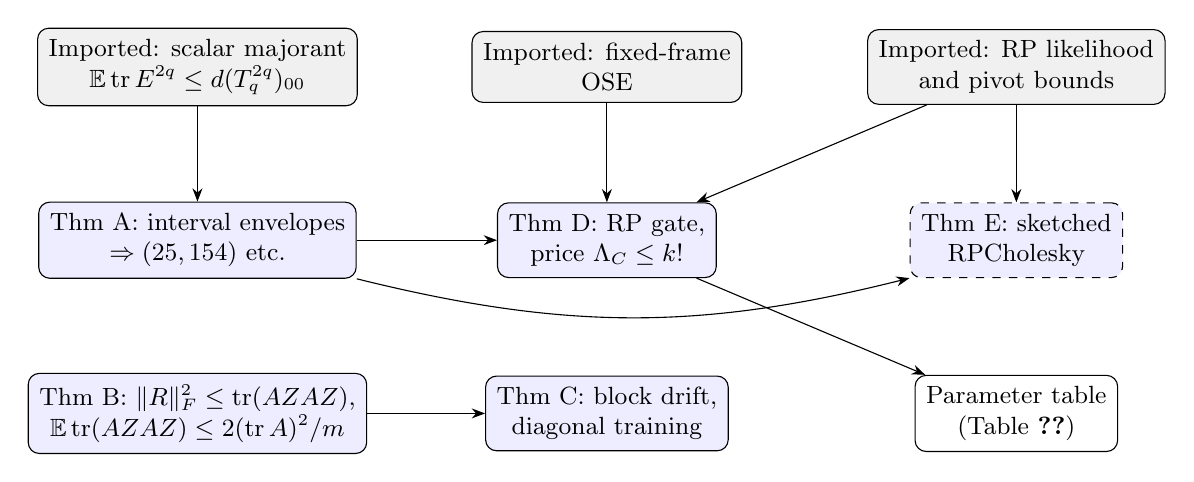
\begin{tikzpicture}[
  box/.style={draw,rounded corners,align=center,font=\small,minimum height=9mm,inner sep=4pt},
  imp/.style={box,fill=gray!12},
  res/.style={box,fill=blue!7},
  >=Stealth]
\node[imp] (maj) at (0,0) {Imported: scalar majorant\\ $\E\tr E^{2q}\le d(T_q^{2q})_{00}$};
\node[imp] (ose) at (5.2,0) {Imported: fixed-frame\\ OSE};
\node[imp] (rpc) at (10.4,0) {Imported: RP likelihood\\ and pivot bounds};
\node[res] (A) at (0,-2.2) {Thm A: interval envelopes\\ $\Rightarrow(25,154)$ etc.};
\node[res] (Cc) at (5.2,-2.2) {Thm D: RP gate,\\ price $\Lambda_C\le k!$};
\node[res,dashed] (Ee) at (10.4,-2.2) {Thm E: sketched\\ RPCholesky};
\node[res] (B) at (0,-4.4) {Thm B: $\norm R_F^2\le\tr(AZAZ)$,\\ $\E\tr(AZAZ)\le2(\tr A)^2/m$};
\node[res] (Cb) at (5.2,-4.4) {Thm C: block drift,\\ diagonal training};
\node[box] (tab) at (10.4,-4.4) {Parameter table\\ (Table~\ref{tab:gate})};
\draw[->] (maj) -- (A);
\draw[->] (ose) -- (Cc);
\draw[->] (rpc) -- (Ee);
\draw[->] (rpc) -- (Cc);
\draw[->] (A) -- (Cc);
\draw[->] (A.south east) to[bend right=14] (Ee.south west);
\draw[->] (Cc) -- (tab);
\draw[->] (B) -- (Cb);
\end{tikzpicture}
\caption{Dependencies. Grey boxes are imported black boxes; blue boxes
are proved here. The dashed box (Theorem~E) is proved in~\cite{RobustRP};
here we supply its SparseStack moment input from Theorem~A. Theorem~B
and Theorem~C use only second and fourth moments of the signed hash
variables.}
\label{fig:roadmap}
\end{figure}

\subsection{Relation to existing work and contribution}
\paragraph{Embedding constants.}
CountSketch originates with Charikar, Chen and
Farach-Colton~\cite{CharikarChenFarachColton2002}. The block construction
used here is that of Kane and Nelson~\cite{KaneNelson2014} and one of
the OSNAP variants of Nelson and Nguyen~\cite{NelsonNguyen2013}.
The name SparseStack and the subspace-injection viewpoint follow
Cama\~no, Epperly, Meyer and Tropp~\cite{CEMT}. Optimal dimension with
near-optimal sparsity was obtained by Chenakkod, Derezi\'nski and
Dong~\cite{CDD2025}. The target dependence on $d,\eps,\delta$ has also
been proved in the SparseStack paper~\cite{SSOriginal} and by Mai and
Rao~\cite{MaiRao2026}. This companion's contribution is the explicit
finite certificate for the three constant pairs in Theorem~A, relative
to the direct certificate of~\cite[Theorem~10.6]{SS}. It does not claim
priority for the construction or for these asymptotic rates.

\paragraph{Approximation and estimation.}
The Nystr\"om projector representation is standard, and the
approximate-matrix-multiplication moment identity is part of sparse
sketching~\cite{ClarksonWoodruff2013,CEMT}. We give a short compression
argument connecting the full Gram error to the squared Frobenius
Nystr\"om residual, together with the exact signed-hash variance and a
finite-support obstruction. These are elementary refinements and
applications of existing mechanisms, rather than a new tail-relative
Nystr\"om theory. The block ratio argument is inherited from the
repository companion~\cite{PPD}; here its exact mixed denominator yields
$\kappa_b=1+2/b$. Stochastic trace and diagonal probing precede this
work~\cite{Hutchinson1989,Bekas2007}, and variance-reduced trace and
diagonal estimators include XTrace and XDiag~\cite{XTrace}. Our
estimation results identify the exact SparseStack variance and the
conditionally unbiased correction from independently sampled diagonals;
we do not claim the probing or control-variate ideas themselves.

\paragraph{Selection after observing the sketch.}
Randomly pivoted Cholesky is due to Chen, Epperly, Tropp and
Webber~\cite{CETW}. The factorial adaptive-versus-volume comparison
is Deshpande and Vempala's Proposition~7~\cite{DV2006}; its proof already
uses residual spectral-tail denominators. We retain those denominators
as the explicit spectral factor $\Lambda_C$, and apply the classical
comparison to transfer fixed-frame guarantees after a sketch-dependent
selection. Thus the new application is the stated sketch-reuse guarantee
and its parameter comparison, not a new factorial sampling theorem.
The fractional likelihood bound is imported from~\cite{RA01}, and
the path-local sketched-RP theorem is imported from~\cite{RobustRP}.
All repository dependencies are identified by their statements and
linked in the bibliography. A literature check supports these bounded
contribution claims; it is not an exhaustive claim of first occurrence.

\section{The SparseStack model and the imported estimates}\label{sec:model}

\begin{definition}[SparseStack]\label{def:ss}
Fix integers $s\ge1$ and $b\ge2$ and put $m=sb$. For $g\in[s]$ and
$i\in[n]$ draw a bucket $h_g(i)$ uniformly from $[b]$ and a Rademacher
sign $\sigma_{gi}$, all $2sn$ variables independent. The CountSketch
block $H_g\in\R^{b\times n}$ has entries
$(H_g)_{ai}=\sigma_{gi}\1\{h_g(i)=a\}$, and
\[
 \Pi=s^{-1/2}\begin{bmatrix}H_1^\T&\cdots&H_s^\T\end{bmatrix}^\T
 \in\R^{m\times n}.
\]
\end{definition}

A direct computation gives the Gram matrix
\begin{equation}\label{eq:gram}
 (\Pi^\T\Pi)_{ij}=\frac1s\sum_{g=1}^s\sigma_{gi}\sigma_{gj}\1\{h_g(i)=h_g(j)\},
 \qquad (\Pi^\T\Pi)_{ii}=1.
\end{equation}
This representation drives Sections~\ref{sec:nystrom}
and~\ref{sec:blocks}. For a fixed isometry $U\in\R^{n\times d}$ write
$E=U^\T\Pi^\T\Pi U-I_d$. Put $h=b-1$ and $r_b=b/(b-1)$.

\subsection{Imported theorems}
We use two results of~\cite{SS} as black boxes. Their exact source is
Theorem~10.6 and Appendix~B.4--B.5 of the repository framework, not the
earlier coupled theorem in \texttt{SparseStack.pdf}~\cite{SSOriginal}.
That earlier paper has a different parameter prescription and a
formal-verification statement for its own theorem. No formal
verification is asserted for the sharper constants proved here.

\begin{imported}[Fixed-frame OSE {\cite[Theorem~10.6]{SS}}]\label{imp:ose}
Let $q,v,D$ be as in Section~\ref{sec:main-results}, $s=\lceil(17/2)v/\eps\rceil$,
$b=\lceil81D/(s\eps^2)\rceil$ and $m=sb$. Then for every isometry
$U\in\R^{n\times d}$, $\Prob\{\norm E>\eps\}\le\delta$. Moreover
$s<26.5\,q/\eps$ and $m<179(d+q)/\eps^2$.
\end{imported}

The second import is the operator part of the proof of
Imported Theorem~\ref{imp:ose}. For even grades $\nu\ge2$ define
\begin{align}
 m\alpha_\nu&=\sqrt{(m+\nu)(d+\nu+1)}+\sqrt{h\nu(d+\nu-1)/2}
   +\nu\sqrt h+\sqrt{bh\nu(\nu-1)/2},\label{eq:alpha}\\
 m\chi_\nu&=d+2\nu-1+2\sqrt{b(\nu-1)(d+\nu-1)}+(\nu+1)\sqrt b+h\nu,
   \label{eq:chi}
\end{align}
and $\alpha_0=\sqrt{(d+1)/m}$, $\chi_0=0$. Let $T_q$ be the symmetric
tridiagonal matrix indexed by $0,\ldots,q$ with diagonal entries
$(T_q)_{kk}=\chi_{2k}$ and off-diagonal entries
$(T_q)_{k,k+1}=(T_q)_{k+1,k}=\alpha_{2k}$.

\begin{imported}[Scalar moment majorant {\cite[Appendix~B.4, equations~(224)--(226)]{SS}}]\label{imp:majorant}
For all integers $n,d,q,s\ge1$, $b\ge2$ and every isometry
$U\in\R^{n\times d}$,
\[
 \E\tr E^{2q}\le d\,(T_q^{2q})_{00}.
\]
The sequence $\nu\mapsto\alpha_\nu$ is increasing on even $\nu\ge0$.
\end{imported}

In~\cite{SS}, the bound comes from an exact multiplication operator on
the signed-bucket probability space, a vacuum moment identity, a
shared-factor light-sector Gram estimate, and block Cauchy--Schwarz
bounds on eight families of local legs; the numbers
$\alpha_\nu,\chi_\nu$ bound the grade-raising and grade-preserving parts
of that operator. Nothing in the present paper reopens these estimates.
The next two lemmas are the elementary scalar steps of~\cite{SS}; we
include their short proofs because Theorem~A applies them to a new
family of envelopes.

\begin{lemma}[Triangular row-sum product]\label{lem:path}
Let $T$ be a nonnegative symmetric tridiagonal matrix indexed by
$0,\ldots,q$ with $T_{00}=0$ and $T_{01}\le a$. Suppose its row sums are
bounded by an increasing sequence $R_0\le R_1\le\cdots\le R_q$. For
$q\ge2$,
\[
 (T^{2q})_{00}\le a^2R_1R_q\prod_{k=2}^{q-1}R_k^2 .
\]
\end{lemma}
\begin{proof}
A nonzero returning walk of length $2q$ starts with the step $0\to1$ and
ends with $1\to0$; these two steps have total weight at most $a^2$.
At time $t$ such a walk sits at an index at most $\min(t,2q-t)$.
Restrict the intermediate states to this range; no contributing walk is
lost. At departure times $t=1,\ldots,2q-2$ the largest permitted row
sums are $R_1,R_2,\ldots,R_q,R_{q-1},\ldots,R_2$. Applying the row-sum
bounds successively to the restricted transition matrices, starting from
the indicator of the final state, bounds the total weight by the product
of these row sums.
\end{proof}

\begin{lemma}[Geometric-mean envelope]\label{lem:gm}
Let $T$ be as in Lemma~\ref{lem:path}, and let $\Psi$ be positive,
increasing and concave on $[0,1]$. Suppose that, for $0\le k\le q$, the
$k$-th row sum of $T/\eps$ is at most $\Psi(u_k)$ with
$u_k=(2k+1)/(2q+1)$, and $T_{01}/\eps\le a$. Put
$J=\exp\int_0^1\log\Psi(u)\,du$. If $a^2J\le\Psi(0)^3$ then, for $q\ge2$,
\[
 (T^{2q})_{00}\le(\eps J)^{2q}.
\]
Moreover, for every $r\ge1$,
\begin{equation}\label{eq:midpoint}
 J\le\Bigl[\prod_{j=0}^{r-1}\Psi\Bigl(\frac{2j+1}{2r}\Bigr)\Bigr]^{1/r}.
\end{equation}
\end{lemma}
\begin{proof}
If $T_{01}=0$ the claim is trivial. Otherwise put $f=\log\Psi$, which is
increasing and concave. Lemma~\ref{lem:path} with $R_k=\eps\Psi(u_k)$
gives
\[
 \tfrac12\log\frac{(T^{2q})_{00}}{\eps^{2q}}
 \le\log a+\tfrac12f(u_1)+\sum_{k=2}^{q-1}f(u_k)+\tfrac12f(1).
\]
The nodes $u_1<\cdots<u_q=1$ have spacing $2/(2q+1)$, so the trapezoidal
sum on the right is at most $(q+\frac12)\int_{u_1}^1f$ by concavity. Since
$(q+\frac12)u_1=\frac32$ and $f\ge f(0)$, this is at most
$q\log J+\frac12\log J-\frac32\log\Psi(0)$. The boundary condition makes
$\log a+\frac12\log J-\frac32\log\Psi(0)\le0$, and exponentiation proves
the first claim. For~\eqref{eq:midpoint}, apply Jensen's inequality to the
concave function $f$ on each of the $r$ intervals $[j/r,(j+1)/r]$.
\end{proof}

For comparison, \cite{SS} applies Lemma~\ref{lem:gm} to one envelope
with $(C,B)=(81,17/2)$, a fixed lower bound $b\ge10$, and the dimension
ratio replaced by one; a four-node midpoint product then certifies
$J<1/2$. The next section refines exactly this last step.

\section{Sharper universal constants}\label{sec:constants}

\begin{theorem}[Refined universal constants]\label{thm:constants}
Let $(C,B)\in\{(69,8),\,(74,15/2),\,(79,7)\}$. With
\[
 s=\Bigl\lceil\frac{Bv}{\eps}\Bigr\rceil,\qquad
 b=\Bigl\lceil\frac{CD}{s\eps^2}\Bigr\rceil,\qquad m=sb,
\]
the SparseStack matrix satisfies, for every $n$ and every isometry
$U\in\R^{n\times d}$,
\[
 \Prob\{\norm{U^\T\Pi^\T\Pi U-I_d}>\eps\}\le\delta.
\]
The parameters obey
\begin{align}
 s&<\frac{2Bq+B+1}{\eps}\le\frac{(3B+1)q}{\eps},\label{eq:s-size}\\
 m&<\frac{Cd+(2C+2B)q+C+B+1}{\eps^2}<\frac{(2C+2B)(d+q)}{\eps^2}.
 \label{eq:m-size}
\end{align}
\end{theorem}

Concretely, the three-term row bound~\eqref{eq:m-size} reads
\[
 \eps^2m<69d+154q+78,\qquad 74d+163q+82.5,\qquad 79d+172q+87,
\]
against $81d+179q+90.5$ for the prescription of~\cite{SS}. The pair
$(69,8)$ minimizes the row constant, $(79,7)$ minimizes the sparsity
constant, and all three improve both constants of $(26.5,179)$. The coefficient of $d$ in the
three-term form is $C$, not $2C+2B$; in the regime $d\gg q$ this is the
relevant constant, and it drops from $81$ to $69$.

The proof occupies the rest of this section. It changes nothing in
Imported Theorem~\ref{imp:majorant}; only the scalar bound on
$(T_q^{2q})_{00}$ is new.

\subsection{Retaining the dimension--bucket relation}\label{sec:retain}
Assume $q\ge2$, so $v\ge5$. Put
\[
 t=\frac vD\in(0,1),\qquad u=\frac{\nu+1}{v},\qquad
 \theta_t(u)=1-t+tu=\frac{d+\nu+1}{D}.
\]
The prescription gives $m\ge CD/\eps^2$ and $s\ge Bv/\eps$.

\begin{lemma}[Bucket lower bounds]\label{lem:bucket}
For $q\ge2$,
\begin{equation}\label{eq:bucket}
 b>\frac CB\qquad\text{and}\qquad b>\frac{C}{t(B+1/5)}.
\end{equation}
\end{lemma}
\begin{proof}
From $s<(Bv+\eps)/\eps$,
\[
 b\ge\frac{CD}{s\eps^2}>\frac{CD}{\eps(Bv+\eps)}.
\]
Since $Bd>1\ge\eps$, we have $BD>Bv+\eps$, so the right side exceeds
$C/(B\eps)\ge C/B$. Also $D=v/t$, so the right side equals
$C/(t\eps(B+\eps/v))\ge C/(t(B+1/5))$, because $\eps\le1$ and $v\ge5$.
\end{proof}

Write $G_b=(2\sqrt{1-1/b}+1)/\sqrt b$. With $y=b^{-1/2}$,
$G_b=2y\sqrt{1-y^2}+y$, whose $y$-derivative
$2(1-2y^2)/\sqrt{1-y^2}+1$ is positive on $[0,1/\sqrt2]$. Hence $G_b$
decreases in $b\ge2$.

\begin{lemma}[Parameter envelope]\label{lem:envelope}
For $q\ge2$ and $1\le k\le q$, the $k$-th row sum of $T_q/\eps$ is at
most $\Phi_{t,b}(u_k)$, $u_k=(2k+1)/v$, where
\begin{equation}\label{eq:Phi}
 \Phi_{t,b}(u)=\frac2{\sqrt C}\sqrt{\Bigl(1+\frac{tu}C\Bigr)\theta_t(u)}
 +\frac{2+\sqrt2}{\sqrt{CB}}\sqrt{u\,\theta_t(u)}
 +\frac{\theta_t(u)}C+\frac{1+\sqrt2+G_b}{B}\,u .
\end{equation}
The row $k=0$ has sum $\alpha_0/\eps$, which is at most half the first
term of $\Phi_{t,b}(u_0)$.
\end{lemma}
\begin{proof}
Fix $\nu=2k\ge2$ and $u=(\nu+1)/v$. Since $\alpha$ increases, the $k$-th
row sum of $T_q$ is at most $2\alpha_\nu+\chi_\nu$. We use
\[
 \frac{d+\nu+1}m\le\frac{\eps^2\theta_t(u)}C,\qquad
 \frac\nu m\le\frac{\nu}{CD}\le\frac{tu}C,\qquad
 \frac hm\le\frac bm=\frac1s\le\frac\eps{Bv},
\]
together with $\eps\le1$ to remove leftover factors $\sqrt\eps$ and
$\eps$. Each group of terms in $(2\alpha_\nu+\chi_\nu)/\eps$ is bounded
as follows.
\begin{enumerate}[leftmargin=2em]
\item Light creation.
 \[\frac{2\sqrt{(m+\nu)(d+\nu+1)}}{m\eps}
 =\frac2\eps\sqrt{\Bigl(1+\frac\nu m\Bigr)\frac{d+\nu+1}m}
 \le\frac2{\sqrt C}\sqrt{\Bigl(1+\frac{tu}C\Bigr)\theta_t(u)}.\]
\item Mixed terms. From $\alpha_\nu$ and from $\chi_\nu$, respectively,
 \begin{align*}
 \frac{2\sqrt{h\nu(d+\nu-1)/2}}{m\eps}&\le\frac2\eps
 \sqrt{\frac{\eps\nu}{2Bv}\cdot\frac{\eps^2\theta_t}{C}}
 \le\sqrt2\sqrt{\frac{u\theta_t}{CB}},\\
 \frac{2\sqrt{b(\nu-1)(d+\nu-1)}}{m\eps}&\le\frac2\eps
 \sqrt{\frac{\eps\nu}{Bv}\cdot\frac{\eps^2\theta_t}C}
 \le2\sqrt{\frac{u\theta_t}{CB}}.
 \end{align*}
\item Heavy creation. $2\sqrt{bh\nu(\nu-1)/2}/(m\eps)\le
 \sqrt2\,b\nu/(m\eps)=\sqrt2\,\nu/(s\eps)\le\sqrt2\,u/B$.
\item Nonradical loops. $d+2\nu-1+h\nu=(d+\nu+1)+(b\nu-2)$, so these
 terms contribute at most $\eps\theta_t/C+\nu/(s\eps)\le\theta_t/C+u/B$.
\item Remaining terms. $2\nu\sqrt h+(\nu+1)\sqrt b\le(\nu+1)bG_b$, so
 they contribute at most $(\nu+1)G_b/(s\eps)\le G_bu/B$.
\end{enumerate}
Summing gives~\eqref{eq:Phi}. For $k=0$ the row sum is
$\alpha_0/\eps=\eps^{-1}\sqrt{(d+1)/m}\le\sqrt{\theta_t(1/v)/C}$.
\end{proof}

The envelope of~\cite{SS} is obtained by replacing $\theta_t$ by $1$ and
$G_b$ by $G_{10}$. Those two losses cannot both be worst-case: when $t$
is small, $\theta_t$ is close to one but Lemma~\ref{lem:bucket} forces
$b$ to be large, and when $t$ is large, $\theta_t$ is visibly smaller
than one. Retaining this correlation is the entire source of the
improvement.

\subsection{A finite family of concave envelopes}\label{sec:intervals}
Partition $(0,1)$ by the $21$ intervals
\[
 [\ell,r]=\Bigl[\frac j{40},\frac{j+1}{40}\Bigr]\quad(0\le j\le19),
 \qquad[\ell,r]=\Bigl[\frac12,1\Bigr].
\]
For each interval put
\begin{equation}\label{eq:nlr}
 n_{\ell,r}=\max\Bigl\{\Bigl\lfloor\frac CB\Bigr\rfloor+1,\;
 \Bigl\lfloor\frac C{r(B+1/5)}\Bigr\rfloor+1\Bigr\},
 \qquad\vartheta_\ell(u)=1-\ell+\ell u,
\end{equation}
and define
\begin{equation}\label{eq:Psi}
 \Psi_{\ell,r}(u)=2\sqrt{\frac{(1+ru/C)\,\vartheta_\ell(u)}C}
 +(2+\sqrt2)\sqrt{\frac{u\,\vartheta_\ell(u)}{CB}}
 +\frac{\vartheta_\ell(u)}C+\frac{1+\sqrt2+G_{n_{\ell,r}}}{B}\,u .
\end{equation}

\begin{lemma}[Interval envelopes]\label{lem:interval}
Let $q\ge2$ and $t=v/D\in[\ell,r]$. Then $b\ge n_{\ell,r}$ and
$\Phi_{t,b}\le\Psi_{\ell,r}$ on $[0,1]$. Each $\Psi_{\ell,r}$ is positive,
increasing and concave on $[0,1]$, and the row sums of $T_q/\eps$ are at
most $\Psi_{\ell,r}(u_k)$ for $0\le k\le q$.
\end{lemma}
\begin{proof}
Since $b$ is an integer, Lemma~\ref{lem:bucket} and $t\le r$ give
$b\ge\lfloor C/B\rfloor+1$ and $b\ge\lfloor C/(r(B+1/5))\rfloor+1$, so
$b\ge n_{\ell,r}$ and $G_b\le G_{n_{\ell,r}}$. For $u\in[0,1]$,
$\theta_t(u)=1-t(1-u)\le1-\ell(1-u)=\vartheta_\ell(u)$ and
$tu\le ru$, which gives $\Phi_{t,b}\le\Psi_{\ell,r}$ termwise. The two
radical terms are geometric means of two nonnegative affine increasing
functions, hence concave and increasing; the other terms are affine and
increasing. The row-sum claim for $k\ge1$ is Lemma~\ref{lem:envelope};
for $k=0$ the row sum is at most half of the first term of
$\Psi_{\ell,r}(u_0)$.
\end{proof}

With the eight midpoint nodes $u_j=(2j+1)/16$, the midpoint
inequality~\eqref{eq:midpoint} gives
\begin{equation}\label{eq:Jlr}
 J_{\ell,r}:=\exp\int_0^1\log\Psi_{\ell,r}(u)\,du
 \le\Bigl[\prod_{j=0}^7\Psi_{\ell,r}(u_j)\Bigr]^{1/8}.
\end{equation}

\begin{proposition}[Exact certificate]\label{prop:cert}
For each of the three pairs $(C,B)$ and each of the $21$ intervals,
$\prod_{j=0}^7\Psi_{\ell,r}(u_j)<2^{-8}$. Consequently
$J_{\ell,r}<1/2$. Table~\ref{tab:cert} lists $n_{\ell,r}$ and integers
$T_{\ell,r}<500000$ with
$\prod_j\Psi_{\ell,r}(u_j)\le(T_{\ell,r}/10^6)^8$.
\end{proposition}
\begin{proof}
Every quantity in~\eqref{eq:Psi} at a rational node is rational except
the square roots. First write
$G_n=(2\sqrt{(n-1)/n}+1)\sqrt{1/n}$, so no radical appears in a
denominator. Replace each square root $\sqrt x$ by the rational
$\lceil10^{12}\sqrt x\rceil/10^{12}$, computed exactly by an integer
square root; this can only increase each factor, since all coefficients
are nonnegative. The resulting rational upper bound $P_{\ell,r}$ of the
eight-factor product is compared with $2^{-8}$, and $T_{\ell,r}$ is the
least integer with $T_{\ell,r}^8\ge10^{48}P_{\ell,r}$, all in exact
integer arithmetic. The program in Appendix~\ref{app:checker} performs
these $63$ checks; its output is Table~\ref{tab:cert}.
\end{proof}

\begin{table}[ht]
\centering\small
\begin{tabular}{l rr rr rr}
\toprule
& \multicolumn{2}{c}{$(69,8)$} & \multicolumn{2}{c}{$(74,15/2)$}
& \multicolumn{2}{c}{$(79,7)$}\\
\cmidrule(lr){2-3}\cmidrule(lr){4-5}\cmidrule(lr){6-7}
Interval $[\ell,r]$ & $n_{\ell,r}$ & $T_{\ell,r}$ & $n_{\ell,r}$ & $T_{\ell,r}$
& $n_{\ell,r}$ & $T_{\ell,r}$\\
\midrule
$[0,1/40]$ & 337 & 497368 & 385 & 496334 & 439 & 497892\\
$[1/40,1/20]$ & 169 & 498517 & 193 & 497515 & 220 & 499113\\
$[1/20,3/40]$ & 113 & 498747 & 129 & 497786 & 147 & 499428\\
$[3/40,1/10]$ & 85 & 498483 & 97 & 497567 & 110 & 499295\\
$[1/10,1/8]$ & 68 & 497916 & 77 & 497122 & 88 & 498824\\
$[1/8,3/20]$ & 57 & 497044 & 65 & 496231 & 74 & 498018\\
$[3/20,7/40]$ & 49 & 496003 & 55 & 495421 & 63 & 497187\\
$[7/40,1/5]$ & 43 & 494796 & 49 & 494096 & 55 & 496151\\
$[1/5,9/40]$ & 38 & 493556 & 43 & 493000 & 49 & 494923\\
$[9/40,1/4]$ & 34 & 492198 & 39 & 491521 & 44 & 493628\\
$[1/4,11/40]$ & 31 & 490609 & 35 & 490208 & 40 & 492191\\
$[11/40,3/10]$ & 29 & 488657 & 33 & 488206 & 37 & 490517\\
$[3/10,13/40]$ & 26 & 487327 & 30 & 486727 & 34 & 488939\\
$[13/40,7/20]$ & 25 & 484934 & 28 & 484852 & 32 & 486990\\
$[7/20,3/8]$ & 23 & 483200 & 26 & 483043 & 30 & 485082\\
$[3/8,2/5]$ & 22 & 480825 & 25 & 480650 & 28 & 483226\\
$[2/5,17/40]$ & 20 & 479259 & 23 & 478951 & 26 & 481438\\
$[17/40,9/20]$ & 19 & 476933 & 22 & 476572 & 25 & 479028\\
$[9/20,19/40]$ & 18 & 474615 & 21 & 474184 & 24 & 476599\\
$[19/40,1/2]$ & 17 & 472308 & 20 & 471789 & 22 & 474954\\
$[1/2,1]$ & 9 & 482285 & 10 & 483066 & 12 & 484537\\
\bottomrule
\end{tabular}
\caption{Exact certificate for Theorem~\ref{thm:constants}: bucket lower
bounds $n_{\ell,r}$ and certified upper bounds $T_{\ell,r}/10^6$ for the
eight-node geometric means $[\prod_j\Psi_{\ell,r}(u_j)]^{1/8}$. Every
entry $T_{\ell,r}$ is below $500000$; the largest is $499428$, for
$(79,7)$ on $[1/20,3/40]$.}
\label{tab:cert}
\end{table}

\begin{figure}[ht]
\centering
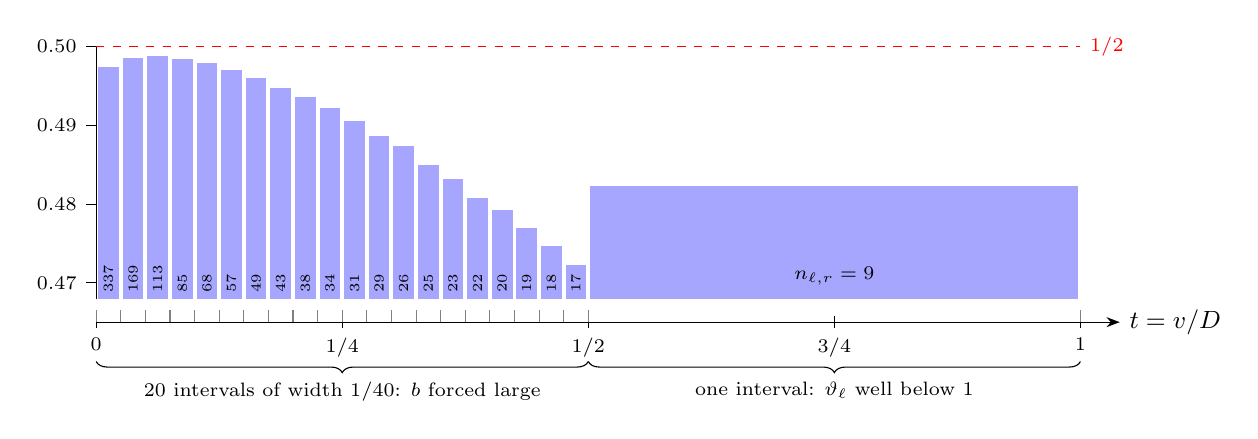
\begin{tikzpicture}[x=12.5cm,y=1cm,>=Stealth]
\def\ymin{0.468}
\draw[->] (0,0) -- (1.04,0) node[right,font=\small] {$t=v/D$};
\foreach \x/\lab in {0/0,0.25/{1/4},0.5/{1/2},0.75/{3/4},1/1}
  \draw (\x,0.08) -- (\x,-0.08) node[below,font=\scriptsize] {$\lab$};
\foreach \j in {0,...,19} \draw[gray] ({\j/40},0) -- ({\j/40},0.15);
\draw[gray] (0.5,0) -- (0.5,0.15); \draw[gray] (1,0) -- (1,0.15);
% bars: (69,8) geometric-mean bounds; height = (T/10^6 - 0.468)*100
\foreach \j/\hh in {0/2.9368,1/3.0517,2/3.0747,3/3.0483,4/2.9916,5/2.9044,
  6/2.8003,7/2.6796,8/2.5556,9/2.4198,10/2.2609,11/2.0657,12/1.9327,
  13/1.6934,14/1.5200,15/1.2825,16/1.1259,17/0.8933,18/0.6615,19/0.4308}
  \fill[blue!35] ({\j/40+0.002},0.3) rectangle ({(\j+1)/40-0.002},{0.3+\hh});
\fill[blue!35] (0.502,0.3) rectangle (0.998,{0.3+(0.482285-\ymin)*100});
\draw[red,dashed] (0,{0.3+(0.5-\ymin)*100}) -- (1,{0.3+(0.5-\ymin)*100})
  node[right,font=\scriptsize,red] {$1/2$};
\draw (0,0.3) -- (0,{0.3+(0.5-\ymin)*100});
\foreach \y in {0.47,0.48,0.49,0.50}
  \draw (0,{0.3+(\y-\ymin)*100}) -- (-0.01,{0.3+(\y-\ymin)*100})
  node[left,font=\scriptsize] {$\y$};
\foreach \j/\nn in {0/337,1/169,2/113,3/85,4/68,5/57,6/49,7/43,8/38,9/34,
  10/31,11/29,12/26,13/25,14/23,15/22,16/20,17/19,18/18,19/17}
  \node[rotate=90,anchor=west,font=\tiny,inner sep=1pt] at ({(\j+0.5)/40},0.33) {\nn};
\node[font=\scriptsize,anchor=south] at (0.75,0.35) {$n_{\ell,r}=9$};
\draw[decorate,decoration={brace,mirror,amplitude=4pt}] (0,-0.5) -- (0.5,-0.5)
  node[midway,below=4pt,font=\scriptsize] {20 intervals of width $1/40$: $b$ forced large};
\draw[decorate,decoration={brace,mirror,amplitude=4pt}] (0.5,-0.5) -- (1,-0.5)
  node[midway,below=4pt,font=\scriptsize] {one interval: $\vartheta_\ell$ well below $1$};
\end{tikzpicture}
\caption{The interval family for $(C,B)=(69,8)$. Bars show the certified
geometric-mean bounds $T_{\ell,r}/10^6$ (axis from $0.468$); numbers inside
the bars are the forced bucket bounds $n_{\ell,r}$. Near $t=0$ the
dimension ratio $\vartheta_\ell$ is close to one, but the buckets are
numerous; near $t=1$ buckets may be few, but $\vartheta_\ell$ is small.}
\label{fig:intervals}
\end{figure}

\subsection{The vacuum boundary condition}\label{sec:vacuum}
Let $t\in[\ell,r]$ and let $a=\alpha_0/\eps$ be the normalized vacuum edge.
Then
\[
 a^2\le\frac{d+1}{CD}=\frac{1-t+t/v}C\le\frac{1-4t/5}{C}
 \le\frac{1-4\ell/5}C,
\]
using $v\ge5$. Put $x=1-\ell\in[1/2,1]$, so $1-4\ell/5=(1+4x)/5$. Since
$J_{\ell,r}<1/2$,
\[
 a^2J_{\ell,r}<\frac{1+4x}{10C}\le\frac{3x}{5C}<\frac{8x^{3/2}}{C^{3/2}}
 \le\Psi_{\ell,r}(0)^3 .
\]
The second inequality is $1+4x\le6x$, i.e.\ $x\ge1/2$. The third is
$3\sqrt C<40\sqrt x$; squaring, it suffices that $9C<800$, which holds
for $C\le79$. The last uses $\Psi_{\ell,r}(0)\ge2\sqrt{\vartheta_\ell(0)/C}=2\sqrt{x/C}$.
Thus the boundary condition of Lemma~\ref{lem:gm} holds for every
interval and every $q\ge2$.

\subsection{Proof of Theorem~\ref{thm:constants}}\label{sec:proof-constants}
\emph{Case $q\ge2$.} Let $t=v/D$ and pick an interval $[\ell,r]$
containing $t$. By Lemma~\ref{lem:interval}, Section~\ref{sec:vacuum} and
Lemma~\ref{lem:gm} with $\Psi=\Psi_{\ell,r}$, together with
Proposition~\ref{prop:cert} and Imported Theorem~\ref{imp:majorant},
\[
 \E\tr E^{2q}\le d\,(T_q^{2q})_{00}\le d(\eps J_{\ell,r})^{2q}
 <d\,(\eps/2)^{2q}.
\]
Since $\norm E^{2q}\le\tr E^{2q}$, Markov's inequality gives
$\Prob\{\norm E>\eps\}<d4^{-q}\le\delta$.

\emph{Case $q=1$.} Here $(T_1^2)_{00}=\alpha_0^2=(d+1)/m\le\eps^2(d+1)/(CD)
\le\eps^2/C$, so $\Prob\{\norm E>\eps\}\le\E\tr E^2/\eps^2\le d/C$.
As $q=1$ forces $d/\delta\le4$, we get $d/C\le4\delta/C\le\delta$.

\emph{Rounding.} Since $s<Bv/\eps+1\le(Bv+1)/\eps$,
$s<(2Bq+B+1)/\eps\le(3B+1)q/\eps$, using $q\ge1$. Next,
$m=sb<s(CD/(s\eps^2)+1)=CD/\eps^2+s$, and with $\eps\le1$,
\[
 \eps^2m<C(d+2q+1)+2Bq+B+1=Cd+(2C+2B)q+C+B+1.
\]
Finally $Cd+C+B+1<(2C+2B)d$ because $(C+2B)d\ge C+2B>C+B+1$ for $B>1$.
This proves~\eqref{eq:s-size} and~\eqref{eq:m-size}. \qed

\begin{remark}[Where the remaining slack lies]\label{rem:slack}
The interval envelopes recover about $6\%$ of the sparsity constant and
$14\%$ of the row constant. A larger reserve sits in the scalar step
itself: Lemma~\ref{lem:path} bounds all returning walks by a product of
row sums. Iterating the tridiagonal majorant $T_q$ directly, with the
prescription of Theorem~\ref{thm:constants}, gives
$(T_q^{2q})_{00}^{1/(2q)}/\eps\approx0.35$ at $(C,B)=(69,8)$ over a
grid reaching $d=10^9$ and $q=3000$, far below the value $1/2$ that the
proof needs; with $(C,B)=(35,8)$ the same diagnostic stays below $0.48$
(Section~\ref{sec:num-majorant}). This suggests the following.
\end{remark}

\begin{conjecture}\label{conj:C35}
With $B=8$ and $C=35$, the prescription of Theorem~\ref{thm:constants}
satisfies $(T_q^{2q})_{00}\le(\eps/2)^{2q}$ for all $d\ge1$, $q\ge2$ and
$0<\eps\le1$. Consequently SparseStack would be an OSE with
$m<(35d+86q+44)/\eps^2$ rows.
\end{conjecture}
A proof would need a sharper bound on returning walks than
Lemma~\ref{lem:path}, for example a diagonal similarity or a Perron
analysis of the continuum limit of $T_q$, certified in exact arithmetic
over a partition in $t$ as above.

\section{A whole-sketch Nystr\"om Frobenius bound}\label{sec:nystrom}

For a PSD matrix $A\in\R^{n\times n}$ and any $\Pi\in\R^{m\times n}$,
the Nystr\"om approximation and its residual are
\[
 \Nys_A(\Pi)=A\Pi^\T(\Pi A\Pi^\T)^+\Pi A,\qquad R=A-\Nys_A(\Pi).
\]
Write $Z=\Pi^\T\Pi-I_n$ for the Gram error of the whole sketch. Unlike an
OSE, which controls $Z$ on one $d$-dimensional subspace, the bounds of
this section see all of $Z$, weighted by $A$.

\begin{theorem}[Deterministic bound]\label{thm:det}
For every PSD $A$ and every $\Pi$,
\[
 0\preceq R\preceq A\qquad\text{and}\qquad
 \norm R_F^2\le\tr(AZAZ)=\norm{A^{1/2}ZA^{1/2}}_F^2 .
\]
\end{theorem}
\begin{proof}
\proofstep{Represent the residual as a compression.}
Let $X=A^{1/2}$ and $K=X\Pi^\T\in\R^{n\times m}$. The matrix
$P=K(K^\T K)^+K^\T$ is the orthogonal projector onto $\range K$, and
$K^\T K=\Pi A\Pi^\T$, $XK=A\Pi^\T$. Hence $XPX=\Nys_A(\Pi)$ and
\[
 R=XQX,\qquad Q=I-P .
\]
This shows $0\preceq R\preceq A$. Since $Q^2=Q$,
\[
 \norm R_F^2=\tr(XQX^2QX)=\tr(QAQA)=\tr(QAQ\cdot QAQ)=\norm{QAQ}_F^2 .
\]
\proofstep{Express the missing part through the Gram error.}
Now $KK^\T=X\Pi^\T\Pi X=A+XZX$ has the same range as $K$, so
$Q(A+XZX)=0$, that is $QA=-QW$ with $W=XZX$ symmetric. Therefore
$QAQ=-QWQ$ and
\[
 \norm R_F^2=\norm{QWQ}_F^2\le\norm W_F^2=\tr(XZX\,XZX)=\tr(AZAZ),
\]
because an orthogonal projector is a contraction on both sides.
\end{proof}

The identity $\norm R_F=\norm{Q(XZX)Q}_F$ inside the proof is exact;
only the compression by $Q$ is dropped. The right side
$\norm{XZX}_F^2=\norm{X^\T\Pi^\T\Pi X-X^\T X}_F^2$ is the squared error of
sketched matrix multiplication for the product $X^\T X=A$.

\subsection{The exact SparseStack computation}
\begin{theorem}[Exact second moment]\label{thm:exact}
Let $\Pi$ be SparseStack with $m=sb$ rows and let $A$ be a fixed symmetric
matrix. Then
\begin{equation}\label{eq:exact}
 \E\tr(AZAZ)=\frac{(\tr A)^2+\norm A_F^2-2\sum_iA_{ii}^2}{m}.
\end{equation}
If $A\succeq0$, then $\E\norm R_F^2\le\E\tr(AZAZ)\le2(\tr A)^2/m$.
\end{theorem}
\begin{proof}
By~\eqref{eq:gram}, $Z_{ii}=0$ and for $i\ne j$
\[
 Z_{ij}=\frac1s\sum_{g=1}^s\sigma_{gi}\sigma_{gj}\1\{h_g(i)=h_g(j)\}.
\]
\proofstep{Compute the pair covariance.}
We claim that the off-diagonal entries have mean zero and variance
$1/m$, and that entries indexed by distinct unordered pairs are
uncorrelated. Indeed $\E Z_{ij}=0$ because $\sigma_{gi}$ is independent
of all other variables in the $g$-th summand. For unordered pairs
$\{i,j\}\ne\{k,l\}$ with $i\ne j$, $k\ne l$, consider a product
$\sigma_{gi}\sigma_{gj}\sigma_{g'k}\sigma_{g'l}$. If $g\ne g'$ it has mean
zero by independence of the blocks. If $g=g'$, some index appears exactly
once among $i,j,k,l$, and the corresponding sign has mean zero and is
independent of the rest, including the hashes. Hence
$\E Z_{ij}Z_{kl}=0$. Finally, cross terms between different blocks
vanish, so
\[
 \E Z_{ij}^2=\frac1{s^2}\sum_{g=1}^s\Prob\{h_g(i)=h_g(j)\}
 =\frac1{s^2}\cdot\frac sb=\frac1m .
\]
\proofstep{Contract the covariance with the matrix.}
Expand the trace as
\[
 \tr(AZAZ)=\sum_{i,j,k,l}A_{li}Z_{ij}A_{jk}Z_{kl}.
\]
The expectation of
$Z_{ij}Z_{kl}$ is nonzero only if $i\ne j$ and $(k,l)\in\{(i,j),(j,i)\}$.
The choice $(k,l)=(j,i)$ contributes $A_{ii}A_{jj}/m$, and $(k,l)=(i,j)$
contributes $A_{ij}^2/m$. Summing over ordered pairs $i\ne j$,
\[
 \E\tr(AZAZ)=\frac1m\Bigl[\sum_{i\ne j}A_{ii}A_{jj}+\sum_{i\ne j}A_{ij}^2\Bigr].
\]
The first sum is $(\tr A)^2-\sum_i A_{ii}^2$; the second is
$\norm A_F^2-\sum_i A_{ii}^2$. Therefore
\[
 \E\tr(AZAZ)=\frac{(\tr A)^2+\norm A_F^2-2\sum_i A_{ii}^2}{m}.
\]
For $A\succeq0$, $\norm A_F^2\le(\tr A)^2$ gives the final bound, and
Theorem~\ref{thm:det} gives $\E\norm R_F^2\le\E\tr(AZAZ)$.
\end{proof}

\begin{remark}[What the bound counts]\label{rem:counts}
The bound $2(\tr A)^2/m$ counts the actual rows $m=sb$ of the sketch,
not the number of blocks, and it does not depend on $s$ and $b$
separately. It is blind to rank: it neither improves when $A$ has low
rank nor involves a tail $\sum_{j>r}\lambda_j(A)$. Only the second-order
structure of $Z$ enters the proof, so the same computation holds whenever
the blocks are independent, the signs in each block are four-wise
independent and independent of the hashes, and the hashes in each block
are pairwise independent. The identity~\eqref{eq:exact} is the classical
sparse-sketch variance of approximate matrix multiplication for $A^{1/2}A^{1/2}$;
a Gaussian sketch with $m$ rows has the larger value
$[(\tr A)^2+\norm A_F^2]/m$, since its diagonal Gram error does not vanish.
\end{remark}

\subsection{No uniform expected tail-relative guarantee}
A natural wish is a bound $\E\norm{R}\le K\,\tau$, where $\tau$ is a
tail of the spectrum of $A$. For a sketch with finitely many values, this
is impossible whenever $m<n$.

\begin{proposition}[Impossibility]\label{prop:impossible}
Let $\Pi$ be a random $m\times n$ matrix with finite support and $m<n$,
and let $1\le r<n$. For every $K<\infty$ there is a PSD $A$ with
\[
 \E\tr R>K\sum_{j>r}\lambda_j(A)\qquad\text{and}\qquad
 \E\norm R_F^2>K\Bigl(\sum_{j>r}\lambda_j(A)\Bigr)^2.
\]
\end{proposition}
\begin{proof}
Pick $\Pi_0$ in the support, with $p_0=\Prob\{\Pi=\Pi_0\}>0$. Since
$m<n$ there is a unit vector $u\in\ker\Pi_0$. For $H>0$ put
$A_H=Huu^\T+I_n$, whose eigenvalues are $H+1,1,\ldots,1$, so
$\sum_{j>r}\lambda_j(A_H)=n-r$ does not depend on $H$. On the event
$\Pi=\Pi_0$ we have $\Pi_0A_H\Pi_0^\T=\Pi_0\Pi_0^\T$ and
$A_H\Pi_0^\T=\Pi_0^\T$, so $\Nys_{A_H}(\Pi_0)=P_0$, the orthogonal
projector onto $\range\Pi_0^\T\perp u$. Hence
$R=Huu^\T+(I-P_0)\succeq(H+1)uu^\T$, and
\[
 \E\tr R\ge p_0(H+1),\qquad\E\norm R_F^2\ge p_0(H+1)^2 .
\]
Letting $H\to\infty$ proves both claims.
\end{proof}

SparseStack has finite support, and for the matrices $A_H$ of the proof
the damage is done on the event $\{\Pi u=0\}$, whose probability is
exponentially small in $s$ for SparseStack (for $u=(e_1-e_2)/\sqrt2$, say,
it equals $(2b)^{-s}$). The proposition therefore rules out uniform
\emph{expected} tail-relative guarantees, but not high-probability
guarantees: a failure budget $\delta$ exceeding the probability of the
bad event absorbs it. For finite-support sketches the right targets
are high-probability statements, such as those obtained from an OSE for
the leading eigenspace, or validated guarantees, in which the error is
estimated a posteriori, for example by the independent diagonal and
trace estimators of Section~\ref{sec:diagtrain}. Rank-blind expected
bounds such as Theorem~\ref{thm:exact} remain possible because they do
not compare with the tail.

\section{Block drift, bucket rows, and diagonal training}\label{sec:blocks}

This section treats sequential Nystr\"om approximation with whole
CountSketch blocks, using the size-biased ratio argument of
\emph{Product-Probe Drift, Kronecker Nystr\"om Approximation, and Trace
Estimation}~\cite{PPD}. Throughout, $H\in\R^{b\times n}$ is one
CountSketch block with independent uniform buckets $h_i\in[b]$ and
independent signs $\sigma_i$, and for a symmetric $M$ we write
$X_M=\tr(HMH^\T)$.

\subsection{Mixed moments and the block ratio}
\begin{lemma}[Mixed trace identity]\label{lem:mixed}
For symmetric $B,R\in\R^{n\times n}$,
\[
 \E X_B=\tr B,\qquad
 \E X_BX_R=\tr B\,\tr R+\frac2b\Bigl(\tr(BR)-\sum_iB_{ii}R_{ii}\Bigr).
\]
If $B,R\succeq0$ then $\E X_BX_R\le\kappa_b\tr B\tr R$ with
$\kappa_b=1+2/b$.
\end{lemma}
\begin{proof}
Expand $X_B=\tr B+\sum_{i\ne j}B_{ij}\sigma_i\sigma_j\1\{h_i=h_j\}$. As in
the proof of Theorem~\ref{thm:exact}, distinct unordered pairs are
uncorrelated and $\E(\sigma_i\sigma_j\1\{h_i=h_j\})^2=1/b$; the two
orderings of a pair give the factor $2$. For PSD matrices
$B_{ii}R_{ii}\ge0$ and $\tr(BR)\le\tr B\tr R$.
\end{proof}

\begin{lemma}[Block ratio]\label{lem:ratio}
Let $B,R\succeq0$ with $\tr B>0$ and $\ker R\subseteq\ker B$, and set
$X_B/X_R=0$ when $X_R=0$. Then
\[
 \E\frac{X_B}{X_R}\ge\frac{(\tr B)^2}{\E X_BX_R}\ge\frac{\tr B}{\kappa_b\tr R}.
\]
\end{lemma}
\begin{proof}
If $X_R=0$ then $R^{1/2}H^\T=0$, so $\range H^\T\subseteq\ker R\subseteq\ker B$
and $X_B=0$. The useful change of measure gives more weight to sketches carrying
more of $B$. Define $d\mathbb Q=X_B\,d\Prob/\tr B$.
Under $\mathbb Q$, $X_R>0$ almost surely. Jensen's inequality for
$x\mapsto1/x$ now gives
\begin{align*}
 \E\frac{X_B}{X_R}
 &=\tr B\,\E_{\mathbb Q}\frac1{X_R}\\
 &\ge\frac{\tr B}{\E_{\mathbb Q}X_R}
 =\frac{(\tr B)^2}{\E X_BX_R}.
\end{align*}
Lemma~\ref{lem:mixed} bounds the denominator and finishes the proof.
\end{proof}

\subsection{Block drift and convex potentials}
For $R\succeq0$ the Nystr\"om update by a fresh block $H$ is
$R'=R-RH^\T(HRH^\T)^+HR$. Updating successively by independent blocks
$H_1,\ldots,H_s$ from $R_0=A$ yields $R_s=A-\Nys_A(Z_s)$ with
$Z_s=[H_1^\T\ \cdots\ H_s^\T]^\T$, because the projector onto
$\range(A^{1/2}Z_s^\T)$ is the sum of the projector onto the previous
range and the projector onto the new part of the range. The normalization
$s^{-1/2}$ of SparseStack does not change the Nystr\"om approximation.

\begin{theorem}[Block drift]\label{thm:block}
For every nonzero $R\succeq0$, $0\preceq R'\preceq R$ and
\[
 \E(\tr R-\tr R')\ge\frac{\tr(R^2)}{\kappa_b\tr R}.
\]
More generally, for every convex $f:[0,\infty)\to[0,\infty)$ with $f(0)=0$,
\begin{equation}\label{eq:convex}
 \E\tr f(R')\le\tr f(R)-\frac{\tr[Rf(R)]}{\kappa_b\tr R}.
\end{equation}
\end{theorem}
\begin{proof}
\proofstep{Lower-bound what the sampled range captures.}
Let $F=R^{1/2}H^\T HR^{1/2}$, and let $P$ be the orthogonal projector
onto $\range F$, which equals $\range(R^{1/2}H^\T)$. Then
$R'=R^{1/2}(I-P)R^{1/2}$, so
$0\preceq R'\preceq R$ and $\tr R-\tr R'=\tr(PR)$. Suppose $X_R=\tr F>0$.
Every eigenvalue of $F$ is at most $\tr F$, so $F/X_R\preceq P$, and for
every $M\succeq0$ commuting with $R$,
\[
 \tr(PM)\ge\frac{\tr(FM)}{X_R}=\frac{X_{R^{1/2}MR^{1/2}}}{X_R}.
\]
With $M=R$ this is $\tr(PR)\ge X_{R^2}/X_R$; with $M=f(R)\succeq0$ it is
$\tr(Pf(R))\ge X_{Rf(R)}/X_R$. Both inequalities also hold when $X_R=0$.
\proofstep{Pass from captured mass to a convex potential.}
Next, $R'$ has the same nonzero eigenvalues as the compression
$(I-P)R(I-P)$. Let $w_1,w_2,\ldots$ be orthonormal eigenvectors of this
compression spanning $\range(I-P)$, with eigenvalues $\mu_k=w_k^\T Rw_k$.
Jensen's inequality for the spectral measure of $R$ in the state $w_k$
gives $f(\mu_k)\le w_k^\T f(R)w_k$, and $f(0)=0$, so
\[
 \tr f(R')\le\sum_kw_k^\T f(R)w_k=\tr f(R)-\tr(Pf(R)).
\]
\proofstep{Average the size-biased ratio.}
Apply Lemma~\ref{lem:ratio} with $B=R^2$ or $B=Rf(R)$; both satisfy
$\ker R\subseteq\ker B$. If $Rf(R)=0$ the claim~\eqref{eq:convex} is
immediate.
\end{proof}

Keeping the exact denominator in Lemma~\ref{lem:ratio} gives the
residual-dependent refinement
\begin{equation}\label{eq:refined-drift}
 \E(\tr R-\tr R')\ge\frac{[\tr(R^2)]^2}
 {\tr(R^2)\tr R+\frac2b\bigl(\tr(R^3)-\sum_i(R^2)_{ii}R_{ii}\bigr)}.
\end{equation}

\begin{corollary}[Independent-block Frobenius bound]\label{cor:blockfrob}
With $T=\tr A>0$ and $s$ independent blocks,
$\E\norm{R_s}_F^2\le\kappa_bT^2/s$.
\end{corollary}
\begin{proof}
Conditionally on $R_t$, Theorem~\ref{thm:block} and $\tr R_t\le T$ give
$\E[\tr R_t-\tr R_{t+1}\mid R_t]\ge\tr(R_t^2)/(\kappa_bT)$. Summing,
$\sum_{t<s}\E\tr(R_t^2)\le\kappa_bT\,\E(\tr R_0-\tr R_s)\le\kappa_bT^2$.
Since $R_{t+1}\preceq R_t$, the sequence $\tr(R_t^2)$ decreases, so
$s\,\E\tr(R_s^2)\le\kappa_bT^2$.
\end{proof}

\begin{remark}[The block bounds lose up to a factor $b$]\label{rem:blockloss}
The proof of Theorem~\ref{thm:block} uses $F\preceq(\tr F)P$, which
credits a $b$-column block with the progress of a single normalized
probe. The bound is tight up to $\kappa_b$ when the residual has rank
one, but for residuals of rank at least $b$ it underestimates the true
progress by a factor of up to about $b$. Monte Carlo ratios of the
observed mean trace drop to the bound $\tr(R^2)/(\kappa_b\tr R)$ are
$4.96$ for $R=I_{12}$, $b=3$; $4.3$ for a $12\times12$ Wishart matrix,
$b=3$; $9.95$ for $R=I_{40}$, $b=8$; and $1.67=\kappa_3$ for a rank-one
$R$ (Table~\ref{tab:nys}). For $A=I_n$, Corollary~\ref{cor:blockfrob} is
nontrivial only for $s>\kappa_bn$ blocks. In contrast, a single block
captures exactly its number of occupied buckets, whose expectation is
$b[1-(1-1/b)^n]$. This calculation exposes the progress lost when an
entire block is credited as one probe; it does not assert guaranteed
full rank at $s=\lceil n/b\rceil$. In the count of sketch columns, the block
guarantees are therefore weaker than whole-sketch or per-column bounds:
Theorem~\ref{thm:exact} gives $2T^2/m=2T^2/(sb)$ where
Corollary~\ref{cor:blockfrob} gives $(b+2)T^2/(sb)$. What the block
argument offers is the explicit constant $\kappa_b$, arbitrary convex
potentials, and the use of independence only across blocks, never within
a block.
\end{remark}

\subsection{The sharp order-one constant of a bucket row}
Spherical probes enjoy entropy-type constants: for a uniformly random
unit vector, $\E X^{1+\beta}$ grows slowly in $\beta$. A single row of a
CountSketch block behaves very differently. Fix a bucket $a$ and
normalize the corresponding row to the isotropic vector
$z_i=\sqrt b\,\sigma_i\1\{h_i=a\}$. For a unit vector $u$ put
$X_u=|u^\T z|^2$.

\begin{proposition}[Bucket rows]\label{prop:bucketrow}
For every unit $u$, $\E X_u=1$ and $\E X_u^2=3+(b-3)\sum_iu_i^4$. If
$b\ge3$ then, for $1\le p\le2$,
\[
 H(p):=\sup_{\norm u=1}\E X_u^p=b^{p-1},
\]
with equality at every coordinate vector $u=e_i$. Consequently the sharp
uniform order-one constant is
$\lim_{\beta\downarrow0}H(1+\beta)^{1/\beta}=b=H(2)$; equivalently
$\sup_{\norm u=1}\E[X_u\log X_u]=\log b$.
\end{proposition}
\begin{proof}
The variables $\sigma_i\1\{h_i=a\}$ are independent, symmetric, with
second moment $1/b$ and fourth moment $1/b$. Hence $\E X_u=\sum_iu_i^2=1$
and
\[
 \E X_u^2=b^2\Bigl[\frac1b\sum_iu_i^4+\frac3{b^2}\sum_{i\ne j}u_i^2u_j^2\Bigr]
 =3+(b-3)\sum_iu_i^4\le b,
\]
using $\sum_iu_i^4\le1$ and $b\ge3$. For $1\le p\le2$, H\"older's
inequality gives
$\E X^p=\E X^{2-p}X^{2(p-1)}\le(\E X)^{2-p}(\E X^2)^{p-1}\le b^{p-1}$.
For $u=e_i$, $X=b$ with probability $1/b$ and $X=0$ otherwise, so
$\E X^p=b^{p-1}$. The limit follows. Finally
$\E[X\log X]=\frac{d}{dp}\E X^p|_{p=1}$, and since $\E X_u^p\le b^{p-1}$
with equality at $p=1$, this derivative is at most $\log b$, with
equality at $u=e_i$.
\end{proof}

Thus the order-one constant of a bucket row equals its worst-case fourth
moment, and spherical entropy constants cannot replace it row by row.
This obstructs one particular transfer; it is not a lower bound on
achievable embedding constants, nor on whole-block progress.

\subsection{Diagonal training and trace estimation}\label{sec:diagtrain}
Let $R\in\R^{n\times n}$ be symmetric and fixed, and let $\Pi$ be an
independent SparseStack with $m_0=s_0b$ rows. From the product
$Y=R\Pi^\T$ form
\[
 h_i=\sum_{a=1}^{m_0}Y_{ia}\Pi_{ai}=(R\Pi^\T\Pi)_{ii}.
\]

\begin{theorem}[Diagonal and trace estimation]\label{thm:diag}
The vector $h$ is unbiased for $\diag R$, and
\[
 \E\norm{h-\diag R}_2^2=\frac{\norm R_F^2-\sum_iR_{ii}^2}{m_0}.
\]
The sketched trace $\sum_ih_i=\tr(\Pi R\Pi^\T)$ is unbiased with
$\operatorname{Var}(\tr\Pi R\Pi^\T)=2(\norm R_F^2-\sum_iR_{ii}^2)/m_0$.
For $t$ independent uniform indices $I_1,\ldots,I_t\in[n]$, also
independent of $\Pi$, the corrected estimator
\[
 \widehat T_R=\sum_ih_i+\frac nt\sum_{\ell=1}^t(R_{I_\ell I_\ell}-h_{I_\ell})
\]
is unbiased for $\tr R$ and
$\operatorname{Var}\widehat T_R\le\frac{n}{m_0t}\bigl(\norm R_F^2-\sum_iR_{ii}^2\bigr)$.
\end{theorem}
\begin{proof}
With $Z=\Pi^\T\Pi-I$, $h_i-R_{ii}=(RZ)_{ii}=\sum_{j\ne i}R_{ij}Z_{ji}$. By
the second-moment structure established in the proof of
Theorem~\ref{thm:exact}, the terms are uncorrelated with variances
$R_{ij}^2/m_0$; summing over $i$ gives the first formula. Next,
$\tr(RZ)=\sum_{i\ne j}R_{ij}Z_{ij}=2\sum_{i<j}R_{ij}Z_{ij}$, whose variance
is $4\sum_{i<j}R_{ij}^2/m_0=2(\norm R_F^2-\sum_iR_{ii}^2)/m_0$.
For $\widehat T_R$, condition on $\Pi$ and write $e_i=R_{ii}-h_i$. The
correction has conditional mean $\sum_ie_i$, so
$\E[\widehat T_R\mid\Pi]=\tr R$ exactly, and
\[
 \operatorname{Var}\widehat T_R=\E\operatorname{Var}(\widehat T_R\mid\Pi)
 \le\E\frac{n^2}{t}\cdot\frac1n\sum_ie_i^2=\frac nt\E\norm{h-\diag R}_2^2 .
\qedhere
\]
\end{proof}

The sketched trace has exactly the variance of Hutchinson's
estimator~\cite{Hutchinson1989} with $m_0$ Rademacher probes, so at second order the sparse SparseStack
probes lose nothing to dense ones. The corrected estimator serves a
different purpose. Given the sketch, $\sum_ih_i$ is a fixed number that
is off by $\tr(RZ)$, whereas $\widehat T_R$ is \emph{conditionally}
unbiased given $\Pi$, and its conditional variance can itself be
estimated from the $t$ sampled indices. This supplies a conditionally unbiased
a-posteriori estimator for a residual such as $R=A-\Nys_A(\Pi_1)$,
whose diagonal entries are cheap when $\diag A$ is available. A
certified confidence interval requires a separate concentration or
sampling-error bound; conditional unbiasedness alone does not provide
one. The training
sketch must be independent of $R$: when $R$ is a Nystr\"om residual from
an earlier sketch $\Pi_1$, a fresh SparseStack is required. A known
low-rank part of $R$ can be added back exactly.

\section{Adaptive frame selection by an RP gate}\label{sec:gate}

An OSE guarantee concerns a subspace fixed before the sketch is drawn.
In applications the subspace is often chosen \emph{after} looking at
the sketch, and independence is lost. A union bound over a dictionary of
$N_{\rm dict}$ candidate frames restores validity at the price of
replacing $\delta$ by $\delta/N_{\rm dict}$. This section shows that when
the choice is made by randomly pivoted Cholesky on a fixed frame, the
price is a likelihood factor that never exceeds $k!$, however large the
dictionary.

\subsection{The gate}
Randomly pivoted Cholesky (RP) on a PSD matrix $M$ picks, at residual
$R$, an index $i$ with probability $R_{ii}/\tr R$ and updates
$R\leftarrow R-R_{:i}R_{i:}/R_{ii}$~\cite{CETW}.

Fix, before the sketch is drawn:
\begin{itemize}[leftmargin=2em]
\item an isometry $V\in\C^{N\times k}$;
\item for every $k$-subset $J\subseteq[N]$ with $\det V_J\ne0$, a target
isometry $U_J$ (for SparseStack, a real $n\times d$ isometry).
\end{itemize}
Here $V_J$ is the $k\times k$ submatrix of rows indexed by $J$. Draw the
sketch $S$ and form a measurable positive-definite $k\times k$ matrix
$C(S)$. Run $k$ fresh RP steps on $VC(S)V^*$, holding $C(S)$ fixed, and
release only the unordered set $J$ of pivots. Finally apply the sketch
$S$ to the selected frame $U_J$. The reference law
\[
 \nu_V(J)=|\det V_J|^2
\]
is a probability distribution by the Cauchy--Binet formula
$\sum_J|\det V_J|^2=\det(V^*V)=1$, and it does not depend on $S$.

\begin{figure}[ht]
\centering
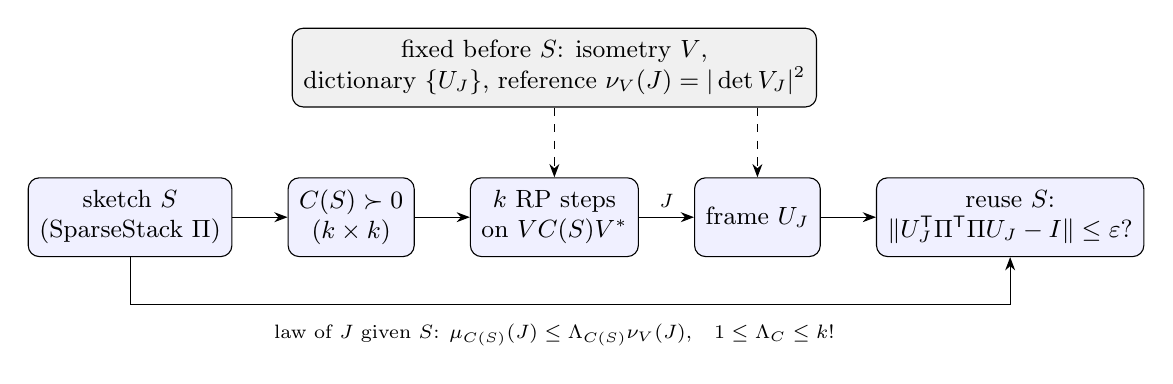
\begin{tikzpicture}[
  box/.style={draw,rounded corners,align=center,font=\small,minimum height=10mm,inner sep=4pt,fill=blue!6},
  fixedb/.style={draw,rounded corners,align=center,font=\small,minimum height=10mm,inner sep=4pt,fill=gray!12},
  >=Stealth, node distance=7mm]
\node[box] (S) {sketch $S$\\ (SparseStack $\Pi$)};
\node[box,right=of S] (Cs) {$C(S)\succ0$\\ ($k\times k$)};
\node[box,right=of Cs] (RP) {$k$ RP steps\\ on $VC(S)V^*$};
\node[box,right=of RP] (J) {frame $U_J$};
\node[box,right=of J] (reuse) {reuse $S$:\\ $\norm{U_J^\T\Pi^\T\Pi U_J-I}\le\eps$?};
\draw[->] (S) -- (Cs);
\draw[->] (Cs) -- (RP);
\draw[->] (RP) -- node[above,font=\scriptsize] {$J$} (J);
\draw[->] (J) -- (reuse);
\draw[->] (S.south) -- ++(0,-0.6) -| (reuse.south);
\node[fixedb] (V) at ($(RP)+(0,1.9)$) {fixed before $S$: isometry $V$,\\ dictionary $\{U_J\}$, reference $\nu_V(J)=|\det V_J|^2$};
\draw[->,dashed] (V) -- (RP);
\draw[->,dashed] (V.south -| J.north) -- (J.north);
\node[font=\scriptsize,align=center] at ($(RP)+(0,-1.5)$)
  {law of $J$ given $S$: $\mu_{C(S)}(J)\le\Lambda_{C(S)}\nu_V(J)$,\quad $1\le\Lambda_C\le k!$};
\end{tikzpicture}
\caption{The gate pipeline. Only the grey data are fixed in advance; the
frame is selected after the sketch is seen, and the same sketch is
reused on the selected frame. The price of the dependence is a bound
$\Lbar$ on the likelihood ratio $\mu_{C(S)}/\nu_V$.}
\label{fig:gate}
\end{figure}

\begin{proposition}[Factorial and spectral prices]\label{prop:gate}
For the eigenvalues $\lambda_1\ge\cdots\ge\lambda_k>0$ of $C$ put
\[
 \tau_j(C)=\sum_{i=j+1}^k\lambda_i\quad(0\le j<k),\qquad
 \Lambda_C=\frac{k!\det C}{\prod_{j=0}^{k-1}\tau_j(C)}.
\]
Conditionally on $S$, the released set has a law $\mu_{C(S)}$ with
\[
 \mu_{C(S)}(J)\le\Lambda_{C(S)}\,\nu_V(J)\quad\text{for all }J,
 \qquad 1\le\Lambda_C\le k!.
\]
Suppose that every fixed target $U_J$ fails, under the law of $S$, with
probability at most $\delta_0$, and that $\Lambda_{C(S)}\le\Lbar$ almost
surely for a deterministic $\Lbar$. Then the selected target $U_J$ fails
with probability at most $\Lbar\delta_0$. In particular,
$\delta_0=\delta/k!$ always suffices.
\end{proposition}
\begin{proof}
\proofstep{Use the classical determinant comparison.}
Write $M=VCV^*$, of rank $k$. For an ordered pivot sequence
$(i_1,\ldots,i_k)$ with set $J$, the product of the pivot diagonals is
the product of the Cholesky pivots of $M_{JJ}$, namely
\[
 \det M_{JJ}=\det(V_JCV_J^*)=\det C\,|\det V_J|^2 .
\]
After $j$ steps, the removed matrix $M-R_j$ is PSD, of rank at most $j$,
and satisfies $M-R_j\preceq M$. By Ky Fan's maximum principle its trace
is at most $\lambda_1+\cdots+\lambda_j$, so $\tr R_j\ge\tau_j(C)$. The
probability of the ordered sequence is therefore at most
$\det C\,\nu_V(J)/\prod_{j<k}\tau_j(C)$. Summing over the at most $k!$
orderings of $J$ gives $\mu_C(J)\le\Lambda_C\nu_V(J)$. Since
$\lambda_{j+1}\le\tau_j(C)\le(k-j)\lambda_{j+1}$, we get
$\det C\le\prod_j\tau_j(C)\le k!\det C$, i.e.\ $1\le\Lambda_C\le k!$.

\proofstep{Transfer fixed-target failure probabilities.}
Let $\mathcal B_J$ be the failure event of the fixed target $U_J$, an
event of $S$ alone. The RP randomness is fresh given $S$, so
\[
 \Prob\{\mathcal B_J\text{ for the selected }J\}
 =\E_S\sum_J\mu_{C(S)}(J)\1_{\mathcal B_J}(S)
 \le\Lbar\sum_J\nu_V(J)\Prob_S(\mathcal B_J)\le\Lbar\delta_0 .
\]
The last step uses only fixed-target guarantees: the weights $\nu_V$
and the targets were fixed before $S$.
\end{proof}

\begin{lemma}[Spectral certificates]\label{lem:bands}
If $C$ is a multiple of $I_k$, then $\Lambda_C=1$. If $C=I+\eta ww^*$
with $\norm w=1$ and $\eta\ge0$, then $\Lambda_C=k(1+\eta)/(k+\eta)$. If
the spectrum of $C$ splits into contiguous bands of sizes $n_\ell$ whose
largest-to-smallest ratios are at most $\rho_\ell$, then
\[
 \Lambda_C\le\min\Bigl\{k!,\;\frac{k!}{\prod_\ell n_\ell!}\prod_\ell\rho_\ell^{n_\ell}\Bigr\};
\]
in particular $\Lambda_C\le k!/\prod_\ell n_\ell!$ when $C$ has exact
eigenvalue levels of multiplicities $n_\ell$.
\end{lemma}
\begin{proof}
For $C=cI$, $\tau_j=(k-j)c$ and $\prod_j\tau_j=k!\,c^k=k!\det C$. For the
spike, $\det C=1+\eta$, $\tau_0=k+\eta$ and $\tau_j=k-j$ for $j\ge1$, so
$\Lambda_C=k!(1+\eta)/((k+\eta)(k-1)!)$. For bands, bound each $\tau_j$
from below by the eigenvalues remaining in its own band: if the $j$-th
index is the $i$-th of band $\ell$, then $\tau_j\ge(n_\ell-i+1)\min_\ell$.
Multiplying, $\prod_j\tau_j\ge\prod_\ell n_\ell!\,(\min_\ell)^{n_\ell}$,
while $\det C\le\prod_\ell(\max_\ell)^{n_\ell}$.
\end{proof}

The gate needs a bound $\Lbar$ that holds uniformly over the permitted
values of $C(S)$. Inserting the observed value $\Lambda_{C(S)}$ into a
failure budget chosen after seeing that same sketch is not justified by
Proposition~\ref{prop:gate}. The argument also does not cover a moving
frame $V(S)$, a sketch-dependent dictionary, partial-rank stopping, or
release of the pivot order.

\subsection{SparseStack parameters after selection}
Proposition~\ref{prop:gate} is distribution-free in $S$: it changes only
the failure allowance of a fixed-frame certificate.

\begin{corollary}[Selected-frame OSE]\label{cor:gate-ss}
In the setting of Proposition~\ref{prop:gate}, let $S=\Pi$ be SparseStack
and let the targets $U_J$ be real $n\times d$ isometries. Replace $q$ by
\[
 q_{\Lbar}=\max\{1,\lceil\log_4(d\Lbar/\delta)\rceil\}
\]
in either the prescription of Imported Theorem~\ref{imp:ose} or that of
Theorem~\ref{thm:constants}. Then
$\Prob\{\norm{U_J^\T\Pi^\T\Pi U_J-I_d}>\eps\}\le\delta$ for the selected $J$.
\end{corollary}
\begin{proof}
With $q_{\Lbar}$, each fixed target fails with probability at most
$d4^{-q_{\Lbar}}\le\delta/\Lbar$ (for $q_{\Lbar}=1$, at most
$d/C\le\delta/\Lbar$); apply Proposition~\ref{prop:gate}.
\end{proof}

For the price $k!$, the extra cost is $\log_4k!$ in $q$, independent of
the dictionary size. Table~\ref{tab:gate} gives exact integer parameters
at $d=100$, $\eps=1/2$, $\delta=0.01$, $k=10$ and $N=1000$, for both
prescriptions.

\begin{table}[ht]
\centering\small
\begin{tabular}{l r rrr rrr}
\toprule
& & \multicolumn{3}{c}{$(C,B)=(81,17/2)$ \cite{SS}}
& \multicolumn{3}{c}{$(C,B)=(69,8)$, Thm.~\ref{thm:constants}}\\
\cmidrule(lr){3-5}\cmidrule(lr){6-8}
Selection price & $q$ & $s$ & $b$ & $m$ & $s$ & $b$ & $m$\\
\midrule
Independent frame, $\Lbar=1$ & 7 & 255 & 147 & 37\,485 & 240 & 133 & 31\,920\\
Two exact levels $5+5$, $\Lbar=252$ & 11 & 391 & 102 & 39\,882 & 368 & 93 & 34\,224\\
Arbitrary spectrum, $\Lbar=10!$ & 18 & 629 & 71 & 44\,659 & 592 & 64 & 37\,888\\
Union bound, $\binom{1000}{10}$ frames & 46 & 1581 & 40 & 63\,240 & 1488 & 36 & 53\,568\\
R\'enyi order $3/2$, $\alpha=\beta/(1+\beta b_k)$ & 72 & 2465 & 33 & 81\,345 & 2320 & 30 & 69\,600\\
R\'enyi order $3/2$, optimal $\alpha$ & 69 & 2363 & 33 & 77\,979 & 2224 & 30 & 66\,720\\
R\'enyi, optimized order (numerical) & 32 & 1105 & 49 & 54\,145 & 1040 & 44 & 45\,760\\
\bottomrule
\end{tabular}
\caption{SparseStack parameters for a frame selected after the sketch, at
$d=100$, $\eps=1/2$, $\delta=0.01$, $k=10$, $N=1000$. The factorial gate
saves $29.4\%$ of the rows and $60.2\%$ of the nonzeros per column
against the union bound; the two-level spectral gate saves more. The
R\'enyi rows use Imported Theorem~\ref{imp:renyi}; see
Section~\ref{sec:renyi}.}
\label{tab:gate}
\end{table}

These are sufficient counts, not measured requirements. Spectral
structure improves the price, but the elementary factorial price alone
already beats the union bound by a wide margin.

\subsection{Why the factorial price beats the R\'enyi price}\label{sec:renyi}
A different route compares $\mu_C$ with the volume law $\nu_V$ through
a R\'enyi divergence. At full rank $k=\rank(VCV^*)$, the
volume-sampling law of $VCV^*$ is exactly $\nu_V$, because
\[
 \frac{\det(VCV^*)_{JJ}}{e_k(VCV^*)}=\frac{\det C\,|\det V_J|^2}{\det C}.
\] The following
bound is proved in \emph{Iterated-logarithmic pivot bounds for randomly
pivoted Cholesky}~\cite{RA01}. For $k\ge2$ and $0<\beta<1$ put
$b_k=\log(1+2\log(k!)/k)$, $a_k=k^k/k!$, and
\[
 B_{k,\beta}(\alpha)=kb_k\alpha-(k-1)\log\alpha,\qquad
 0<\alpha\le\beta .
\]
The argument of~\cite{RA01} is valid for every $0<\alpha\le\beta$; the
minimizing choice is $\alpha_{k,\beta}=\min\{\beta,(k-1)/(kb_k)\}$, and we
write $B_{k,\beta}=B_{k,\beta}(\alpha_{k,\beta})$.

\begin{imported}[Fractional likelihood moment {\cite{RA01}}]\label{imp:renyi}
Let $L=\mu/\nu$ be the likelihood ratio of the $k$-step RP set law to
the volume law of a PSD matrix of rank at least $k$. For $p=1/\beta>1$,
\[
 \E_\nu L^p\le e^{pB_{k,\beta}}\,2^k\,a_k^{\,p}.
\]
The same bound holds with $B_{k,\beta}(\alpha)$ in place of $B_{k,\beta}$
for every $0<\alpha\le\beta$.
\end{imported}

H\"older's inequality gives, for every event $\mathcal E$,
$\mu(\mathcal E)\le(\E_\nu L^p)^{1/p}\nu(\mathcal E)^{1-1/p}$. Apply it
conditionally on $S$ to $\mathcal E_S=\{J:\text{the fixed target }U_J
\text{ fails on }S\}$, and then average over $S$ using the concavity of
$x\mapsto x^{1-1/p}$ and $\E_S\nu_V(\mathcal E_S)\le\delta_0$: the selected
target fails with probability at most
$(\sup_C\E_\nu L_C^p)^{1/p}\delta_0^{1-1/p}$. At $p=3/2$
this is at most $\delta$ once
\[
 \log\frac1{\delta_0}=3\log\frac1\delta+\mathfrak d_k,\qquad
 \mathfrak d_k=3B_{k,2/3}+2k\log2+3\log a_k .
\]
The factorial gate instead needs $\log(1/\delta_0)=\log(1/\delta)+\log k!$.
Both prices grow faster than linearly in $k$, but differently:
\[
 \log k!=k\log k-k+O(\log k),\qquad
 \mathfrak d_k=k\bigl(6+2\log2+3\log b_k\bigr)+O(\log k),
\]
since $B_{k,\beta}=k(1+\log b_k)+O(\log k)$ at the optimal $\alpha$ and
$\log a_k=k-O(\log k)$. The R\'enyi price is linear in $k$ up to the
triply-logarithmic factor $\log b_k$, but with a large constant, and it
also triples $\log(1/\delta)$. The factorial price wins as long as
$\log k-1<6+2\log2+3\log b_k$, that is, while $\log k$ is below about
$12$. Exact evaluation at $\delta=0.01$ places the crossover at
$k\approx1.33\times10^5$ with the optimal $\alpha$ and at
$k\approx1.66\times10^5$ with the simpler admissible choice $\alpha=\beta/(1+\beta b_k)$.
At $k=10$ the R\'enyi price is $\log(1/\delta_0)\approx90$ nats against
$19.7$ for the factorial price, which explains the last rows of
Table~\ref{tab:gate}.

\begin{remark}[Optimizing the R\'enyi order]\label{rem:renyi-order}
H\"older's inequality works for every $p>1$, with
$\log(1/\delta_0)=\frac p{p-1}\log\frac1\delta+\frac1{p-1}\log\E_\nu L^p$.
Numerically optimizing over $p$ in Imported Theorem~\ref{imp:renyi}, the
best order is near $p\approx6.6$ at $k=10$ and gives $q=32$, still far
worse than the factorial gate. With the order optimized separately for
each $k$, the R\'enyi price drops below the factorial price from about
$k\approx130$ on (at $\delta=0.01$). For selector ranks in the tens the
elementary factorial gate is the right tool; for large $k$ a
likelihood-moment bound is preferable.
\end{remark}

\section{Sketched RPCholesky with SparseStack}\label{sec:sketchedrp}

Let $F\in\R^{p\times n}$ be a data matrix with Gram matrix $A=F^\T F$,
fix a target rank $r\ge1$, and put
\[
 \tau=\tau_r(A)=\sum_{j>r}\lambda_j(A)>0,\qquad \eta_A=\frac\tau{\tr A}.
\]
\emph{Sketched RP} draws a SparseStack $\Pi$, runs $k$ steps of RP on the
sketched Gram $\widehat A=(\Pi F)^\T(\Pi F)$, and returns the pivot set $J_k$
together with the regression coefficients $\widehat X=(\Pi F_J)^+\Pi F$. The
point is that $\widehat A$ is formed from the $m\times n$ matrix $\Pi F$, never
from $F$ itself. For a pivot set $J$ write $R_A(J)$ and $R_{\widehat A}(J)$
for the Schur-complement residuals of $A$ and $\widehat A$; the true error
is the residual trace $\tr R_A(J)=\norm{F-P_{F_J}F}_F^2$ of the selected
columns. In this section $\eps\in(0,1]$ denotes the target accuracy of RP;
the distortion of the sketch is written $2\eps_0$.

The frame of interest is chosen by the sketch, so a fixed-frame OSE does
not apply directly, and the gate of Section~\ref{sec:gate} does not fit
either: at full rank it is trivial, and at partial rank it is outside
its hypotheses. The result below shows that RP needs embeddings only of
the $(k+1)$-dimensional frames that it actually meets along its pivot
path, and that these frames can be handled through the exact
likelihood of the path.

\begin{lemma}[Moment bound at every order]\label{lem:moment-any-q}
Let $(C,B)$ be one of the pairs of Theorem~\ref{thm:constants}, let
$q\ge2$ and $0<\eps\le1$, and let $s=\lceil B(2q+1)/\eps\rceil$,
$b=\lceil C(d+2q+1)/(s\eps^2)\rceil$. Then every isometry $U$ with
$d'\le d$ columns satisfies $\E\tr(U^\T\Pi^\T\Pi U-I_{d'})^{2q}<d'(\eps/2)^{2q}$.
\end{lemma}
\begin{proof}
The case $d'=d$ is the case $q\ge2$ of the proof of
Theorem~\ref{thm:constants}, which does not use the relation between $q$
and $\delta$. For $d'<d$, the numbers $\alpha_\nu,\chi_\nu$
of~\eqref{eq:alpha}--\eqref{eq:chi} increase with $d$, so $T_q$ for $d'$
is entrywise at most $T_q$ for $d$, and Imported
Theorem~\ref{imp:majorant} gives
$\E\tr E^{2q}\le d'(T_q^{2q})_{00}<d'(\eps/2)^{2q}$.
\end{proof}

The following consequence uses the fixed-state comparison, hybrid
argument and determinant route of \emph{RPCholesky under approximate
and sketched pivot probabilities}~\cite{RobustRP}. We state the basic
trace recurrence, specialize its moment input to SparseStack, and
record explicitly the moment order required by that determinant route.

\begin{imported}[Sketched RPCholesky {\cite{RobustRP}}]\label{thm:sketchedrp}
Let $0<\eta\le1/4$, put $\gamma=(1-\eta-\eta^2)/(1+\eta)$, let
$0<\eps_0\le\eta/2$ and $q\ge\max\{2,k\}$, and let $\Pi$ be SparseStack with the
prescription of Lemma~\ref{lem:moment-any-q} at dimension $d=k+1$, with
$2\eps_0$ in place of $\eps$.
Let $\varphi_\gamma(x)=x-\gamma(x-\tau)_+^2/(rx)$. Then:
\begin{enumerate}[leftmargin=2em,label=(\roman*)]
\item $\E\tr R_A(J_k)\le\varphi_\gamma^{\circ k}(\tr A)+\tr A\cdot P_{\rm fail}$;
\item $P_{\rm fail}\le\sum_{t=1}^k(1-\eta-\eta^2)^{-t}\sqrt t\,(1+\eps_0)^t\sqrt{\delta_1}$,
 where $\delta_1\le(3k+4)2^{-q}$ bounds the failure probability of the
 good event below for any fixed pivot set of size at most $k$;
\item on the good event at $J_k$,
 $\norm{F-F_J\widehat X}_F^2\le\bigl(1+\eta^2/(2(1-\eta)^2)\bigr)\tr R_A(J_k)$.
\end{enumerate}
In particular, for $0<\eps\le1$, the choices
$k\ge(r/\gamma)\bigl(1/\eps+\log(1/\eps)+\log(1/\eta_A)\bigr)$
and $q=O(k+\log(1/(\eps\eta_A)))$, with $\eps_0=\eta/2$, give
$\E\tr R_A(J_k)\le(1+2\eps)\tau$, with
\[
 m=O\Bigl(\frac{k+\log(1/(\eps\eta_A))}{\eta^2}\Bigr)
\]
rows, independent of $n$ and of $\rank F$. For $k<n$, if the sketched
residual trace reaches zero before $k$ pivots, continue with an arbitrary
unselected index until the budget is used; the theorem concerns this
completed rule. A premature zero state is a failure unless the true
residual is also zero. If $k\ge n$, selecting all original columns and
using the exact refit gives zero error.
\end{imported}

\paragraph{Proof outline: establish one fixed-state event.}
For a fixed set $J$ let $Q_J$ be an orthonormal basis of $\range F_J$,
let $E_J=(I-Q_JQ_J^\T)F$ be the true residual, and let $W_J$ be the
diagonal matrix of drift weights $\norm{R_Ae_i}^2/(R_A)_{ii}$, taking
the weight to be zero when the denominator is zero. For each nonzero
column $m_i$ of $M=E_J$ or $M=E_JW_J^{1/2}$, set
$u_i=m_i/\norm{m_i}$ and
$Z_i=[Q_J,u_i]^\T\Pi^\T\Pi[Q_J,u_i]-I$.
The good event $G(J)$ requires the embedding of $Q_J$ with error at
most $\eta$ and, for each of these two matrices, the weighted bound
\[
 \Phi(M)=\sum_{i:m_i\ne0}\frac{\norm{m_i}^2}{\norm M_F^2}
                    \norm{Z_i}^4\le\eta^4/4.
\]
For $M=0$ this condition is automatic. Jensen's inequality implies
that $\norm{\Pi M}_F^2$ lies within $(1\pm\eta)\norm M_F^2$ and
$\norm{Q_J^\T\Pi^\T\Pi M}_F^2\le(\eta^2/2)\norm M_F^2$.
Minkowski's inequality in $L^{q/2}$ and Markov's inequality give
\[
 \Prob\{G(J)^c\}\le(k+1)(4^{-q}+2\cdot2^{-q})
                  \le(3k+4)2^{-q}=:\delta_1.
\]
Each frame has dimension at most $k+1$; the weighted averages avoid a
union bound over columns.

\paragraph{Turn that event into true-residual progress.}
On $G(J)$ the identity
$\tr R_{\widehat A}(J)=\norm{\Pi E_J}_F^2-\norm{P_{\Pi F_J}\Pi E_J}_F^2$ gives
$(1-\eta-\eta^2)\tr R_A\le\tr R_{\widehat A}\le(1+\eta)\tr R_A$, and the same identity
applied to $E_JW_J^{1/2}$ shows that the sketched step decreases the true
residual trace by at least $\gamma\tr(R_A^2)/\tr R_A$ in expectation. \paragraph{Control the first failed state along the path.}
A hybrid process that follows sketched RP until the first bad state and
exact RP afterwards obeys the $\gamma$-recurrence, and Jensen's inequality
for the concave map $\varphi_\gamma$ gives~(i). For~(ii), the exact path
identity
\[
 \frac{\mathrm{pr}_\Pi(w)}{\mathrm{pr}(w)}=\det(Q_J^\T\Pi^\T\Pi Q_J)\prod_{j<t}
 \frac{\tr R_A(J_j)}{\tr R_{\widehat A}(J_j)},
\]
for an ordered pivot path $w$ of length $t$ with prefix sets $J_j$ and
final set $J$, compares the sketched path law $\mathrm{pr}_\Pi$ with the
exact RP path law $\mathrm{pr}$,
which does not depend on $\Pi$; it holds because the product of pivot
diagonals equals a determinant. Cauchy--Schwarz with
$\E\det(Q_J^\T\Pi^\T\Pi Q_J)^2\le t(1+\eps_0)^{2t}$ then bounds the
probability that the first failure occurs at step $t$. This uses
the $2q$-th Gram-error moment to control a determinant of degree $t$,
and requires $t\le q$. Lemma~\ref{lem:moment-any-q} supplies the actual
frame-dimension prefactor $t$, giving the displayed $\sqrt t$ factor.
The stronger hybrid likelihood bound
in~\cite{RobustRP} dispenses with the restriction $q\ge k$.

\paragraph{Recover the same-sketch regression error.}
Write $F_J=QT$ with $Q=Q_J$ and $T$ of full row rank, and let
$E=E_J$. On the good event, $G=Q^\T\Pi^\T\Pi Q$ is invertible. The
prediction, rather than the coefficient matrix, satisfies
\[
 F_J\widehat X=QQ^\T F+QG^{-1}Q^\T\Pi^\T\Pi E.
\]
The two residual components are orthogonal because $Q^\T E=0$.
Consequently the excess squared error is
$\norm{G^{-1}Q^\T\Pi^\T\Pi E}_F^2$, which yields~(iii).

\begin{remark}
The row count must grow with the pivot budget $k$, not only with $r$:
RP on $\widehat A$ stops after $\rank\widehat A\le m$ pivots. Numerically, sketched RP
with $m=2k$ SparseStack rows already matches exact RP closely
(Section~\ref{sec:num-sketchedrp}); the provable constants are far more
conservative because of the $e^{O(k)}$ likelihood factor in~(ii).
\end{remark}

\section{Numerical diagnostics}\label{sec:numerics}

The diagnostics in this section are numerical evidence, not proofs.
The original scripts and recorded outputs are supplied in this paper's
\texttt{checks/} directory. They were run in Julia~1.13; majorant
computations use 128--256-bit floating point, Nystr\"om and diagonal
experiments use $2\times10^4$--$4\times10^4$ trials, gate experiments
enumerate all pivot paths, and the final sketched-RP experiment uses
$150$ trials per setting. Only the exact rational certificate of
Proposition~\ref{prop:cert} enters a proof.

An independent Python check, supplied as
\texttt{checks/independent\_audit.py}, reproduces all $63$ rational
certificates and the integer parameter table, enumerates $64$ small
CountSketch matrices to verify the moment and drift calculations, and
enumerates full-rank RP laws on $48$ complex instances. Its separate
log-domain majorant propagation reproduces the displayed maxima
$0.352$ and $0.477$ for $C=69$ and $C=35$. These finite numerical
checks supplement the analytic arguments; they do not establish the
open all-order conjecture.

\subsection{Headroom in the scalar majorant}\label{sec:num-majorant}
With the prescription of Theorem~\ref{thm:constants} and varying $C$
at $B=8$, we built $T_q$ from~\eqref{eq:alpha}--\eqref{eq:chi} and
iterated it in high precision, computing $\rho=(T_q^{2q})_{00}^{1/(2q)}/\eps$
over $d\in\{1,10,10^2,10^4,10^6,10^8\}$, $q\in\{2,5,10,40,100,200\}$ and
$\eps\in\{1,1/2,1/20\}$; for $C\in\{69,35\}$ the grid was extended to
$d\in\{10,10^3,10^6,10^9\}$ and $q\in\{200,1000,3000\}$ at $\eps=1$.
The proof needs $\rho<1/2$. The worst values
occur at $\eps=1$ and large $d$:
\begin{center}\small
\begin{tabular}{lccccc}
\toprule
$(C,B)$ & $(81,17/2)$ & $(69,8)$ & $(40,8)$ & $(35,8)$ & $(30,8)$\\
\midrule
$\max\rho$ & $0.319$ & $0.352$ & $0.441$ & $0.477$ & $0.505$\\
\bottomrule
\end{tabular}
\end{center}
At $(C,B)=(69,8)$ the envelope certificate is tight
($T_{\ell,r}/10^6\le0.4988$), while the majorant itself sits near $0.35$.
The threshold $1/2$ is crossed between $C=30$ and $C=35$, which motivates
Conjecture~\ref{conj:C35}. On a grid of $d\le10^6$, $q\le40$ and five
values of $\eps$, the row sums of $T_q/\eps$ never exceeded
$\Phi_{t,b}(u_k)$, in agreement with Lemma~\ref{lem:envelope}.

\subsection{Nystr\"om and drift experiments}\label{sec:num-nys}
Table~\ref{tab:nys} compares, for SparseStack, the Monte Carlo mean of
$\tr(AZAZ)$ with formula~\eqref{eq:exact}, the realized
$\E\norm R_F^2$, and the two upper bounds $2(\tr A)^2/m$
(Theorem~\ref{thm:exact}) and $\kappa_b(\tr A)^2/s$
(Corollary~\ref{cor:blockfrob}). The deterministic inequality
$\norm R_F^2\le\tr(AZAZ)$ held in every trial. The lower part of the
table gives the one-block drift experiments of
Remark~\ref{rem:blockloss}.

\begin{table}[ht]
\centering\small
\begin{tabular}{lccccc}
\toprule
Matrix, $(s,b)$ & MC $\tr(AZAZ)$ & formula~\eqref{eq:exact} &
$\E\norm R_F^2$ & $2(\tr A)^2/m$ & $\kappa_b(\tr A)^2/s$\\
\midrule
$A_{30}$, $(4,6)$ & 0.568 & 0.568 & $<10^{-4}$ & 1.019 & 4.077\\
Wishart $12\times12$, $(3,4)$ & 8.103 & 8.059 & 0.043 & 16.445 & 49.334\\
$I_{20}$, $(2,5)$ & 37.988 & 38.000 & 10.116 & 80.000 & 280.000\\
\midrule
One block, drift & observed & bound & ratio & &\\
\midrule
$R=I_{12}$, $b=3$ & 2.978 & 0.600 & 4.96 & &\\
Wishart $12\times12$, $b=3$ & 4.272 & 0.993 & 4.30 & &\\
$R=I_{40}$, $b=8$ & 7.963 & 0.800 & 9.95 & &\\
rank one, $n=12$, $b=3$ & 1.000 & 0.600 & 1.67 & &\\
\bottomrule
\end{tabular}
\caption{Monte Carlo diagnostics ($2\times10^4$ trials) for
Sections~\ref{sec:nystrom} and~\ref{sec:blocks}, with
$A_{30}=G\diag(0.7^j)G^\T/30$. ``Bound'' is
$\tr(R^2)/(\kappa_b\tr R)$ from Theorem~\ref{thm:block}. For $I_{20}$
with $m=10$, $\norm R_F^2=20-\rank\Pi\ge10$, so the rank-blind bound
cannot be small there.}
\label{tab:nys}
\end{table}

The diagonal-training formula of Theorem~\ref{thm:diag} was checked on
a $12\times12$ Wishart matrix with $(s_0,b)=(3,4)$: Monte Carlo mean
squared error $0.6045$ against the exact value $0.6036$
($4\times10^4$ trials).

\subsection{The gate}\label{sec:num-gate}
Exhaustive enumeration of the full-rank RP set law on $VCV^*$ for $40$
random complex instances ($N\in\{4,5,6\}$, $k\in\{2,3\}$, random
isometry $V$ and random positive-definite $C$) gave
$\max_J\mu_C(J)/(\Lambda_C\nu_V(J))=0.961$, consistent with
Proposition~\ref{prop:gate}; equality $\mu_C=\nu_V$ holds for flat $C$.
The spike formula of Lemma~\ref{lem:bands} was confirmed at $k=10$,
$\eta=3$: $\Lambda_C=40/13\approx3.077$.

\subsection{Factorial versus R\'enyi prices}\label{sec:num-price}
Figure~\ref{fig:price} plots the ratio of the two failure-allowance
costs, $[3\log(1/\delta)+\mathfrak d_k]/[\log(1/\delta)+\log k!]$ at
$\delta=0.01$, using the optimal $\alpha$ in $B_{k,2/3}$. The factorial
gate is cheaper as long as the ratio exceeds one.

\begin{figure}[ht]
\centering
\begin{tikzpicture}[x=1.9cm,y=1.2cm,>=Stealth]
\draw[->] (0,0) -- (6.4,0) node[right,font=\small] {$\log_{10}k$};
\draw[->] (0,0) -- (0,5.4) node[above,font=\small] {cost ratio R\'enyi\,/\,factorial};
\foreach \x in {0,1,...,6} \draw (\x,0.05) -- (\x,-0.05) node[below,font=\scriptsize] {$\x$};
\foreach \y in {1,2,3,4,5} \draw (0.05,\y) -- (-0.05,\y) node[left,font=\scriptsize] {$\y$};
\draw[red,dashed] (0,1) -- (6.2,1) node[above left,font=\scriptsize,red] {break-even};
\draw[thick,blue!70!black] plot[mark=*,mark size=1.2pt] coordinates {
 (0.301,4.15) (0.699,4.907) (1,4.577) (1.301,3.897) (1.699,3.081) (2,2.62)
 (2.477,2.101) (3,1.723) (3.477,1.48) (4,1.283) (4.477,1.145) (5,1.025)
 (5.114,1.002) (5.301,0.967) (6,0.855)};
\draw[->,font=\scriptsize] (5.12,2.1) node[above] {$k\approx1.33\times10^5$} -- (5.12,1.08);
\node[font=\scriptsize,anchor=west] at (1.05,4.75) {$k=10$: $90.2$ vs $19.7$ nats};
\end{tikzpicture}
\caption{Ratio of the R\'enyi-order-$3/2$ cost to the factorial cost of
the failure allowance, $\delta=0.01$ (numerical evaluation of exact
formulas). Below $k\approx1.3\times10^5$ the elementary $k!$ price is
cheaper.}
\label{fig:price}
\end{figure}

\subsection{Sketched RPCholesky}\label{sec:num-sketchedrp}
We took $F=U\Sigma V^\T\in\R^{300\times400}$ with Haar factors, five
unit singular values and $295$ squared singular values in
$[2.5,5]\times10^{-6}$, so $r=5$ and $\eta_A\approx2.2\times10^{-4}$, and
compared exact RP on $A=F^\T F$ with RP on $(\Pi F)^\T(\Pi F)$ for a
SparseStack with $s=4$ blocks and for a Gaussian sketch, $150$ trials
each. The table reports $\E\tr R_A(J_k)/\tau$ and the mean ratio of the
same-sketch regression error $\norm{F-F_J\widehat X}_F^2$ to $\tr R_A(J_k)$.
\begin{center}\small
\begin{tabular}{lccccc}
\toprule
& exact RP & SparseStack RP & Gaussian RP & regression ratio & $1+\frac k{m-k-1}$\\
\midrule
$k=10$, $m=20$ & 1.610 & 1.632 & 1.624 & 1.98 & 2.11\\
$k=10$, $m=40$ & 1.610 & 1.664 & 1.645 & 1.34 & 1.35\\
$k=20$, $m=40$ & 1.195 & 1.201 & 1.199 & 1.98 & 2.05\\
$k=20$, $m=80$ & 1.195 & 1.196 & 1.199 & 1.33 & 1.34\\
\bottomrule
\end{tabular}
\end{center}
Already at $m=2k$ the sketched pivots are within a few percent of exact
ones, whereas the same-sketch regression pays roughly the
Gaussian factor $1+k/(m-k-1)$. Selecting pivots is therefore much less
demanding than solving the sketched regression, which is consistent with
the path-local structure of Imported Theorem~\ref{thm:sketchedrp}.

\section{Open problems}\label{sec:open}

\begin{enumerate}[leftmargin=2em,label=\arabic*.]
\item \emph{The scalar step.} Prove Conjecture~\ref{conj:C35}, or any
bound on returning walks of $T_q$ sharper than the row-sum product of
Lemma~\ref{lem:path}. The diagnostics of
Section~\ref{sec:num-majorant} suggest that the operator estimates of
the imported theorems already support a row constant near $86$ in the
form $(2C+2B)$, and a $d$-coefficient near $35$. A certificate would
likely combine a diagonal similarity of $T_q$ with an exact interval
partition in $t=v/D$, as in Section~\ref{sec:intervals}.

\item \emph{Block progress at the right scale.} Replace $\tr F$ by
$\lambda_{\max}(F)$ in the proof of Theorem~\ref{thm:block}, through a
block-level size-biased ratio controlled by a mixed moment of the top
eigenvalue of $HRH^\T$, so that a $b$-column block is credited with
progress proportional to $\min(b,\rank R)$ probes.

\item \emph{Tail-relative high-probability Nystr\"om bounds.}
Proposition~\ref{prop:impossible} excludes uniform expected
tail-relative guarantees for finite-support sketches with $m<n$.
Determine the sharp high-probability dependence of
$\norm{A-\Nys_A(\Pi)}$ on the tail for SparseStack, in terms of $m$, $s$
and $\delta$, without passing through an OSE for the leading
eigenspace.

\item \emph{A useful selection rule with a fixed range.}
Proposition~\ref{prop:gate} requires the frame $V$ and the dictionary to
be fixed in advance and the selection to be full rank. Find natural
selection rules in which a sketch-dependent $C(S)$ carries real
information while $V$ stays fixed, or extend the likelihood argument to
partial-rank stopping.

\item \emph{Gate prices between $k!$ and R\'enyi.} For $10\le k\le10^5$,
neither the factorial nor the R\'enyi price is sharp. A pointwise
likelihood bound that interpolates between $k!$ and
$\exp(O(k\log\log\log k))$, possibly using the spectrum of $C(S)$ as in
Lemma~\ref{lem:bands}, would lower $q$ for moderate selector ranks.

\item \emph{Sketched RP constants.} The likelihood factor $e^{O(k)}$ in
Imported Theorem~\ref{thm:sketchedrp}(ii) makes the provable row count about
$10^3$--$10^4\cdot k$ at constant $\eta$, while
Section~\ref{sec:num-sketchedrp} shows $m=2k$ working in practice. Remove
the exponential factor, for instance by a martingale argument along the
pivot path.
\end{enumerate}

\appendix
\section{The certificate checker}\label{app:checker}
The following self-contained Julia program (standard library only)
reproduces Proposition~\ref{prop:cert} and Table~\ref{tab:cert}.
All arithmetic is exact: \texttt{Rational\{BigInt\}} throughout, each
square root is replaced by an upper bound $\lceil10^{12}\sqrt x\rceil/10^{12}$
obtained from an integer square root and verified by squaring, and the
final comparisons are integer comparisons. An integer bisection finds $T_{\ell,r}$, so no floating-point
operation enters the certificate. The program prints one line per pair and
interval and ends with \texttt{certificate valid: true}.

In words, for each of the $3\times21$ cases the program:
(1) computes $n_{\ell,r}$ from~\eqref{eq:nlr};
(2) evaluates the upper-rounded envelope~\eqref{eq:Psi} exactly at the
eight nodes $u_j=(2j+1)/16$ and multiplies the values into $P_{\ell,r}$;
(3) checks $P_{\ell,r}<1/256$;
(4) finds the least integer $T$ with $T^8\ge10^{48}P_{\ell,r}$ and checks
$T<500000$; and (5) checks the vacuum condition $9C<800$.

\begin{lstlisting}[language={}]
# Exact certificate for the interval envelopes Psi_{l,r}: every radical is
# rounded up to a rational with denominator K; everything else is exact.
const K = big(10)^12
function sqrt_up(x::Rational{BigInt})              # a rational >= sqrt(x)
    N, D = numerator(x) * K^2, denominator(x)
    k = isqrt(cld(N, D))
    while k * k * D < N; k += 1; end
    return k // K
end
const S2 = sqrt_up(big(2) // 1)
G_up(n) = (2 * sqrt_up((n - 1) // n) + 1) * sqrt_up(1 // n)
function Psi_up(u, l, r, C, B, n)
    th = 1 - l + l * u
    2 * sqrt_up((1 + r * u / C) * th / C) + (2 + S2) * sqrt_up(u * th / (C * B)) +
        th / C + (1 + S2 + G_up(n)) * u / B
end
bucket(C, B, r) = max(floor(BigInt, C / B), floor(BigInt, C / (r * (B + 1 // 5)))) + 1
intervals = [[(big(j) // 40, big(j + 1) // 40) for j in 0:19]; (big(1) // 2, big(1) // 1)]
pairs = [(big(69) // 1, big(8) // 1), (big(74) // 1, big(15) // 2), (big(79) // 1, big(7) // 1)]
nodes = [big(2j + 1) // 16 for j in 0:7]
ok = true
for (C, B) in pairs, (l, r) in intervals
    n = bucket(C, B, r)
    P = prod(Psi_up(u, l, r, C, B, n) for u in nodes)   # >= prod of Psi(u_j)
    lo, hi = big(0), big(500000)
    while hi - lo > 1
        mid = (lo + hi) >> 1
        if mid^8 >= P * big(10)^48; hi = mid; else; lo = mid; end
    end
    T = hi                    # least T with (T/1e6)^8 >= P, if P < 1/256
    global ok &= (P < big(1) // 256) && (T < 500000) && (9C < 800)
    println("C=$C B=$B [$l,$r] n=$n T=$T")
end
println("certificate valid: ", ok)
\end{lstlisting}

\begin{thebibliography}{99}

\bibitem{CEMT}
C.~Cama\~no, E.~N. Epperly, R.~A. Meyer, and J.~A. Tropp.
\newblock Faster linear algebra algorithms with structured random matrices.
\newblock arXiv:2508.21189, 2025. \url{https://arxiv.org/abs/2508.21189}.

\bibitem{CharikarChenFarachColton2002}
M.~Charikar, K.~C. Chen, and M.~Farach-Colton.
\newblock Finding frequent items in data streams.
\newblock In \emph{ICALP 2002}, LNCS 2380, pages 693--703. Springer, 2002.

\bibitem{CETW}
Y.~Chen, E.~N. Epperly, J.~A. Tropp, and R.~J. Webber.
\newblock Randomly pivoted {C}holesky: Practical approximation of a kernel
  matrix with few entry evaluations.
\newblock \emph{Comm. Pure Appl. Math.}, 78(5):995--1041, 2025.
\newblock \url{https://arxiv.org/abs/2207.06503}.

\bibitem{ClarksonWoodruff2013}
K.~L. Clarkson and D.~P. Woodruff.
\newblock Low rank approximation and regression in input sparsity time.
\newblock In \emph{STOC 2013}, pages 81--90. ACM, 2013.
\newblock \url{https://arxiv.org/abs/1207.6365}.

\bibitem{DV2006}
A.~Deshpande and S.~Vempala.
\newblock Adaptive sampling and fast low-rank matrix approximation.
\newblock In \emph{APPROX/RANDOM 2006}, LNCS 4110, pages 292--303, 2006.
\newblock Full version: ECCC Report TR06-042, Proposition~7.
\newblock \url{https://eccc.weizmann.ac.il/report/2006/042/}.

\bibitem{RA01}
\newblock Iterated-logarithmic pivot bounds for randomly pivoted {C}holesky.
\newblock Repository manuscript, 2026.
\newblock \href{https://github.com/DiarHaidary/Results/blob/main/manuscripts/background/Iterated_Logarithmic_RPCholesky.pdf}{PDF in this repository}.

\bibitem{PPD}
\newblock Product-probe drift, {K}ronecker {N}ystr\"om approximation, and
  trace estimation.
\newblock Repository companion, 2026.
\newblock \href{https://github.com/DiarHaidary/Results/blob/main/manuscripts/02-Product-Probe-Drift/Product_Probe_Drift_v2.pdf}{PDF in this repository}.

\bibitem{RobustRP}
\newblock {RPC}holesky under approximate and sketched pivot probabilities.
\newblock Repository companion, 2026.
\newblock \href{https://github.com/DiarHaidary/Results/blob/main/manuscripts/06-Robust-Sketched-RPCholesky/RPCholesky_Approximate_Sketched_Pivots.pdf}{PDF in this repository}.

\bibitem{SS}
\newblock Graded multiplication operators for random-matrix moments.
\newblock Repository manuscript, 2026. Theorem~10.6; Appendix~B,
  equations~(224)--(226), pages~137--139.
\newblock \href{https://github.com/DiarHaidary/Results/blob/main/Graded\%20Multiplication\%20Operators\%20for\%20Random-Matrix\%20Moments.pdf}{PDF in this repository}.

\bibitem{SSOriginal}
D.~Heidary.
\newblock SparseStack is an optimal oblivious subspace embedding.
\newblock arXiv:2609.02978, 2026. The repository's earlier coupled
  version has a different constant prescription.
\newblock \href{https://arxiv.org/abs/2609.02978}{arXiv};
  \href{https://github.com/DiarHaidary/Results/blob/main/SparseStack.pdf}{earlier repository PDF}.

\bibitem{MaiRao2026}
T.~Mai and A.~Rao.
\newblock The Nelson--Nguyen conjecture via mean-to-moments concentration.
\newblock arXiv:2609.22548, 2026.
\newblock \url{https://arxiv.org/abs/2609.22548}.

\bibitem{CDD2025}
S.~Chenakkod, M.~Derezi\'nski and X.~Dong.
\newblock Optimal oblivious subspace embeddings with near-optimal sparsity.
\newblock \emph{ICALP 2025}, LIPIcs 334, Article 55.
\newblock \url{https://doi.org/10.4230/LIPIcs.ICALP.2025.55}.

\bibitem{Hutchinson1989}
M.~F. Hutchinson.
\newblock A stochastic estimator of the trace of the influence matrix
  for Laplacian smoothing splines.
\newblock \emph{Communications in Statistics--Simulation and
  Computation}, 18(3):1059--1076, 1989.
\newblock \url{https://doi.org/10.1080/03610918908812806}.

\bibitem{Bekas2007}
C.~Bekas, E.~Kokiopoulou and Y.~Saad.
\newblock An estimator for the diagonal of a matrix.
\newblock \emph{Applied Numerical Mathematics}, 57:1214--1229, 2007.
\newblock \url{https://doi.org/10.1016/j.apnum.2007.01.003}.

\bibitem{XTrace}
E.~N. Epperly, J.~A. Tropp and R.~J. Webber.
\newblock XTrace: Making the most of every sample in stochastic trace estimation.
\newblock \emph{SIAM Journal on Matrix Analysis and Applications},
 45(1):1--23, 2024.
\newblock \url{https://arxiv.org/abs/2301.07825}.

\bibitem{KaneNelson2014}
D.~M. Kane and J.~Nelson.
\newblock Sparser {J}ohnson--{L}indenstrauss transforms.
\newblock \emph{J. ACM}, 61(1):4:1--4:23, 2014.
\newblock \url{https://doi.org/10.1145/2559902}.
\newblock Preprint: \url{https://arxiv.org/abs/1012.1577}.

\bibitem{NelsonNguyen2013}
J.~Nelson and H.~L. Nguyen.
\newblock {OSNAP}: Faster numerical linear algebra algorithms via sparser
  subspace embeddings.
\newblock In \emph{FOCS 2013}, pages 117--126. IEEE, 2013.
\newblock \url{https://arxiv.org/abs/1211.1002}.

\end{thebibliography}

\end{document}
